\documentclass{article}[12pt,subeqn]

%================================================================================
%PACKAGES
%================================================================================
\usepackage{amsmath}
%\usepackage{appendix}
\usepackage{array}
\usepackage{booktabs}
%\usepackage{cleveref}
\usepackage[usenames, dvipsnames]{color} 
\usepackage{framed}
\usepackage[capposition=top]{floatrow}
\usepackage[pdftex]{graphicx}
\usepackage[update,prepend]{epstopdf}
\usepackage{hyperref}
\usepackage[utf8]{inputenc}
%\usepackage{lineno}
\usepackage{lscape}
\usepackage{natbib}
\usepackage{rotating,capt-of}
\usepackage{setspace}
\usepackage{subfloat}
\usepackage{subcaption}
\usepackage[capposition=top]{floatrow}
\usepackage{zref-xr}
\zexternaldocument{onlineAppendix}


\bibliographystyle{abbrvnat}
\bibpunct{(}{)}{;}{a}{,}{,}



%================================================================================
%TITLE
%================================================================================
\title{Maternal Education and Maternal Mortality: 
Evidence from a Large Panel and Various Natural Experiments}
\author{Sonia Bhalotra\thanks{Department of Economics, The University of Essex,
    Colchester UK. Contact: srbhal@essex.ac.uk}
  \and{Damian Clarke\thanks{Department of Economics, The University of Santiago
      de Chile. Contact: damian.clarke@usach.cl}}}
\date{\today}


%================================================================================
%MARGINS
%================================================================================
\setlength\topmargin{-0.375in}
\setlength\textheight{8.8in}
\setlength\textwidth{5.8in}
\setlength\oddsidemargin{0.4in}
\setlength\evensidemargin{-0.5in}
\setlength\parindent{0.25in}
\setlength\parskip{0.25in}



%================================================================================
%NEW COMMANDS
%================================================================================
\newcommand{\Lagr}{\mathcal{L}}
\newcommand{\vect}[1]{\mathbf{#1}}
\newcolumntype{P}[1]{>{\raggedright}p{#1\linewidth}}
%\newcommand{\MMRfolder}{"/home/damiancclarke/investigacion/Activa/MMR"}
\newcommand{\MMRfolder}{"."}

\hypersetup{                                                                                                    
    colorlinks=true,   
    linkcolor=BlueViolet,
    citecolor=BlueViolet,
    filecolor=BlueViolet,
    urlcolor=BlueViolet
}  



\begin{document}
\begin{spacing}{1.4}

\maketitle

%================================================================================
%ABSTRACT
%================================================================================
\begin{abstract}
We examine whether a causal relationship exists between maternal education and 
maternal mortality. Despite a large body of evidence in favour of a causal 
relationship between education and a range of other health behaviours and 
outcomes, and a significant gradient between maternal mortality and education 
across time and countries, no comprehensive study exists to examine whether this 
relationship is---at least in part---causal.  By forming a large panel of data 
consisting of 108 countries over 20 years, and by examining three natural 
experiments resulting in plausibly exogenous expansions in education, we present 
evidence from various contexts to suggest that increases in maternal education
causally reduce the likelihood of dying in childbirth.  The size of this
relationship is considerable.  Our preferred estimates suggest that moving from 0
to 1 years of education will reduce rates of maternal death in childbirth by 171
deaths per 100,000 live births, while moving from 7 to 8 years results in a
smaller, but still significant, 15 fewer deaths per 100,000 live births.  Turning
to mechanisms, we find that it is female, rather than male, education that
matters for reducing maternal deaths, and that additionally, the \emph{relative}
level of women's to men's education has important predictive power.  Where women
have similar levels of education to men, differentials in desired fertility
between husbands and wives are reduced, with flow-on effects to maternal deaths.
\end{abstract}
\hspace{8mm} \textbf{JEL codes:} H52, I15, I18, J13.

\newpage
%================================================================================
%INTRODUCTION
%================================================================================
\section{Introduction}
Life expectancy exhibits a consistently positive gradient in education that, 
unlike income gradients, tends not to diminish as education levels rise, and is 
evident across and within rich and poor countries \citep{RichardsBarry1998, 
KunstMackenbach1994, EloPreston1996, LlerasMuney2005, Mearaetal2008}. Maternal 
mortality is an important determinant of life expectancy for women in developing 
countries but there is relatively little evidence of the relationship between
maternal mortality and education. This paper attempts to fill that gap.

Every day, approximately 800 women die from preventable causes related to 
pregnancy and childbirth with 99\% of all maternal deaths occuring in
developing countries \citep{WHO2012}. The maternal mortality ratio in developing
countries is 240 per 100,000 births versus 16 per 100,000 in developed countries.
There are large disparities between and within countries, with a few countries
having extremely high maternal mortality ratios of 1,000 or more per 100,000 live
births; more than half of all maternal deaths occur in sub-Saharan Africa and
almost one third occur in South Asia \citep{WHO2012}. The WHO identifies poverty,
limited access to public services, cultural practices and lack of information as
the main causes or sources of variation in maternal mortality ratios. 

However policy documents on maternal mortality seldom indicate education as a 
cause and the academic literature has very little to say about the relationship 
between maternal mortality and education. This said,
there is a lively literature in economics that documents a positive correlation 
between education and other indicators of health. One possibility, relatively 
uninteresting for policy, is that this correlation is driven by time preference, 
where people with lower discount rates tending to invest more in both forms of
human capital. While this is likely so, the crop of studies that identify causal 
effects of education on health most often tend to associate this with educated 
people engaging in healthier behaviours, for instance, smoking and drinking
less and being more likely to seek prenatal care, adopt new drugs or adhere to 
treatment for disease \citep{GoldmanSmith2010, GoldmanLakdawalla2001, 
CurrieMoretti2003, LichtenburgLlerasMuney2005, CutlerLlerasMuney2010,
GliedLlerasMuney2010, JensenLlerasMuney2012}. This is consistent with the 
efficacy that education confers in acquiring and processing relevant information 
\citep{Rosenzweig1995, RosenzweigSchultz1989, CutlerLlerasMuney2010}. Education 
may also influence health through its influence on income and, thereby, the 
facility to purchase health inputs, but the impacts of education on health tend
to be larger than the direct impacts of income, to hold conditional upon income,
and to be similar for men and women, at least in richer countries
\citep{LlerasMuney2005, CutlerLlerasMuney2010}.

The proximate causes of maternal mortality are pregnancy complications such as 
pre-eclampsia, bleeding, infections and unsafe abortion.\footnote{We provide a
more extensive discussion of the medical literature related to maternal mortality
and death in and surrounding childbirth in online appendix A.} To 
the extent that educated women are more likely to adopt simple and low-cost 
practices to maintain hygiene, are more able to react to symptoms such as bleeding 
or high blood pressure, more likely to assess the information on abortion and place 
of abortion, and more willing to accept
treatment and birth attendance, education may plausibly cause declines in maternal 
mortality. Moreover, if these are the mechanisms by which it acts, then education 
may have an impact on maternal mortality conditional upon the state of health 
services. The payoff to education tends to be higher in circumstances where 
learning is important, for instance, circumstances of structural and technological 
change \citep{FosterRosenzweig2004}. Such change is characteristic of developing 
countries which, in the post-war period, have experienced massive technological 
change in the public health sphere \citep{Cutleretal2006} as well as changes in 
the economic (and occupational) structure.

Using panel data for 108 developing countries and new estimates of maternal 
mortality ratios for 1990-2010, we begin by estimating the relationship between
maternal mortality and educational attainment under the standard panel data
identifying assumptions, unconditional and conditional upon indicators of income,
public health provision and fertility. We find large and consistently significant
impacts of education. Indeed, depending upon the specification, the (standardized)
impacts of education on maternal mortality are equal to or larger than the impacts
of skilled birth attendance, an instrument that the WHO currently focuses upon in 
devising programs to address maternal mortality. In contrast, within-country 
variation in GDP has no significant impact on maternal mortality conditional upon 
education. We supplement the cross-country analysis with quasi-experimental case 
studies from Nigeria, Zimbabwe and Kenya. These are three countries that 
implemented substantial education reforms. We use cohort and region variation in 
education generated by the reform, which we argue is plausibly exogenous. To match 
this to maternal mortality rates, we construct cohort mortality rates for regions 
within these countries using the Demographic and Health Surveys. In two of the 
three case we identify a sizeable and negative impact of improvements in education 
on maternal mortality. In both Nigeria and Zimbabwe we find that the educational 
expansions due to policy experiments significantly reduce maternal death in
affected cohorts, and find that these results are surprisingly close to those 
estimated in cross-country regressions.  In Kenya---which experienced a schooling 
extension at the lower high school level---we do not find evidence of such a 
reduction, estimating that the effect on maternal mortality is not significantly 
different to zero.

We then consider the mechanisms underlying the effect of education on maternal
mortality.  We document that reductions in maternal mortality are due nearly
entirely to changes in female rather than male education, and that educational
attainment of fertile aged women is the most important in predicting declines in
maternal deaths. We then test whether \emph{relative} education of women and men
is important, conditional on women's education itself.  We find that the ratio
of men's to women's education has considerable predictive power, both in terms
of the likelihood that a husband desires more children than his wife, and the
total number of maternal deaths.  This result is consistent with a situation in
which a woman's bargaining power in the household affects fertility choices and
maternal mortality, in line with current and ongoing work of
\citeauthor{Ashrafetal2012} (\citeyear{Ashrafetal2012,Ashrafetal2014}).

All in all, this paper generates new data on maternal mortality that is available 
for individuals within regions and states of countries, and it provides what would 
appear to be the first systematic consideration of the relationship between 
maternal mortality ratios and education. It opens up several avenues for further 
research.

%================================================================================
%METHODOLOGY
%================================================================================
\section{Methodology}
\subsection{Cross-Country Analysis}
In order to examine the effect of educational expansions on maternal mortality, 
we run country-level regressions of the following form:
\begin{equation}
\label{eqn:panel}
   MMR_{ct}=\mathbf{educ}_{ct}\beta + \mathbf{W}_{ct}\gamma+\alpha_c+\alpha_t+
   \varepsilon_{ct},
\end{equation}
where $MMR_{ct}$ refers to the maternal mortality rate in country $c$ and period 
$t$, $\mathbf{educ}_{ct}$ to a series of variables measuring the percent of the 
population with a given level of education, and $\mathbf{W}_{ct}$ refers to a 
vector of relevant country- and time-varying covariates.  Given that we have both 
temporal and regional variation in the variables of interest, we employ a 
fixed-effects methodology which allows for us to control for all time-fixed 
country-specific factors which may confound the analysis in (\ref{eqn:panel}).%
\footnote{As a robustness test, we include country-specific linear time trends
$\alpha_c\cdot t$ in all regressions.}
The ability to eliminate these time invariant factors is particularly important 
in this analysis given that many unobserved factors, such as the institutional 
and political aspects of a given country, are likely to be correlated with both 
maternal mortality and educational attainment. Whilst some of these variables are 
not strictly ``time-invariant'', they evolve sufficiently slowly that our analysis 
over a comparatively short time horizon will mean that a fixed-effect estimator 
will largely control for them. We cluster standard errors at the level of the 
country (allowing for the stochastic term $\varepsilon_{ct}$ to be correlated over
time for each $c$.)\footnote{In certain cases when we restrict to only certain
  sub-groups of countries, the number of countries in each regression is less than
  50.  Rule of thumb-type considerations suggest that clustering standard errors
  using less than around 50 clusters is not optimal \citep{AngristPischke2009,
    NicholsSchaffer2007}. In these cases we also estimate using heteroscedasticity
  robust standard errors, and wild bootstrapped standard errors
  \citep{MackinnonWebb2014,CameronMiller2015}. To be conservative, we always
  report the set of estimates with the largest standard errors (on our variables of
  interest).}

We estimate (\ref{eqn:panel}) for a number of different subgroups. Whilst we
primarily focus on women of reproductive age, our data allows us to run a similar
analysis for educational attainment of both gender groups and for various age
subgroups created within the fertile age range. We also segregate countries by
region- and income-level, and present group-specific estimates of the above
specification. A full list of the educational variables which we use and a 
description of the time varying covariates $\textbf{W}_{ct}$ is provided in
section \ref{scn:data}. 

\subsection{Natural Experiments}
\label{scn:empiricalexperiment}
In addition to (\ref{eqn:panel}) which we estimate with country by year panel
data, we focus on a number of country-specific cases in countries which have
experienced isolated, policy-defined expansions in schooling achievement. Such
expansions allow for us to causally identify the effect of education on maternal
mortality if we believe that we can identify similar subgroups of individuals
who are differentially affected by these isolated shocks to education. In these
country case studies, we construct comparable subgroups of women who entered
school on either side of an important educational reform.  We exploit variation
in the intensity of treatment between regions and cohorts of birth to estimate
the effect of educational expansions on maternal mortality.

Prominent educational reforms discussed in the economics literature are listed 
in table \ref{MMRtab:EducExp}.  Of the reforms listed here, we identify 
three which are suitable to use as natural experiments to identify the effect of 
education on maternal mortality.  These are Nigeria, Zimbabwe, and Kenya. Of the 
other three cases listed, they were either not examined as they occurred too 
recently to observe the outcome of interest (maternal mortality) or because 
microdata for maternal mortality outcomes was not available for the country in 
question. For each of the three natural experiments examined, we briefly describe 
the nature of the reform, and the identification strategy used in estimation.

\subsubsection{Nigeria 1976}
\label{ssscn:empiricsNigeria}
The Universal Primary Education (UPE) program was initiated in Nigeria in 
September 1976 as a national program directed at primary school enrolment. This 
program involved the provision of free primary school education, along with 
significant classroom construction \citep{OsiliLong2008}. The gross primary 
enrolment rate doubled between 1974 and 1981 for male students, and nearly 
tripled for females.  \citet{OsiliLong2008} suggest using a double-differences 
identification strategy in which women from cohorts born between 1970 and 1975 in 
high-intensity states\footnote{Prior to the UPE program the non-Western states of 
Nigeria had low primary enrolment rates and low levels of investment per capita.  
With the introduction of the UPE, these states experienced a considerable 
expansion in educational investments \citep{OsiliLong2008}, and so are defined as 
`high-intensity' states.} act as the treatment group. As per 
\citeauthor{OsiliLong2008}, rather than opt for a control group immediately older 
than the treatment group, we examine women born between 1956-1961 in order for our 
analysis to not be confounded by over- and under-age enrolments in primary school.  
We also examine the effect on cohorts born between 1965 and 1970, which may be 
partially affected by the reform given over-age enrolment in primary school.

Two measures of treatment intensity are defined: a dummy for those living in 
high-intensity states, and a measure of federal capital funds dispersed per capita 
in each state in 1976 (the year of the reform)\footnote{Two additional treatment 
measures are examined by interacting funds per capita with treatment state, and 
funds per capita with number of years affected by the treatment. Further details 
are available as notes to Table \ref{MMRtab:Nigeria}.}.  The effect of UPE on 
schooling and maternal mortality is then estimated using a difference-in-difference 
framework:
\begin{equation}
 \label{eqn:Nigeria}
  y_{ijk}=\alpha + \beta \text{ UPE Cohort}_{jk}+\gamma \text{UPE Input}_k+
   \delta(\text{UPE Input}_k\times\text{UPE Cohort}_{jk})+
   \textbf{X}^\prime_{ijk}\theta+\varepsilon_{ijk}.
\end{equation}
The schooling and maternal mortality outcomes ($y$) for individual $i$ in cohort 
$j$ and state $k$ are regressed on controls for year of birth, religion, 
ethnicity, and additional controls for groups differentially affected by the 
1967-`70 civil war (see \citet{Akreshetal2012} for further discussion.)  The UPE 
Cohort dummy captures whether an individual was of primary school age at the time 
of the reform (year of birth between 1970 and 1975 inclusive), and UPE Input is a 
dummy for whether an invididual resides in a high-intensity treatment state, or 
the investment per capita of a given individual's state as discussed above.  For 
educational outcomes we expect that $\delta$---the reduced form estimate of the 
effect of UPE---should be positive, and, if education reduces maternal mortality, 
that $\delta<0$ for maternal mortality outcomes.  Further details and summary 
statistics for outcome and treatment variables are provided in section 
\ref{scn:data}.

\subsubsection{Zimbabwe 1980}
\label{ssscn:empiricsZimbabwe}
\citet{AgueroBharawadj2011} use extensions of schooling availability to black 
citizens in 1980 after independence in Zimbabwe to isolate the effect of 
education on health investments. This extension in years of education was 
observed in high-school age students, with the authors demonstrating a 
discontinuity between the ages of 14 and 15.  The reform in question occurred in 
April 1980, and has been used in the literature in earlier papers (see for 
example \citet{Edwards1995}).

In isolating the effect of the reform we follow \citet{AgueroBharawadj2011} in 
estimating around the discontinuity in educational attainment between the cohorts 
aged 14 and 15 in 1980: 
\begin{equation}
\label{eqn:Zimbabwe}
    y_{ij}=\beta_1\text{DumAge}_{ij}+
    \beta_2\text{DumAge}_{ij}\times(\text{Age}80_{ij}-14)+
    \beta_3(1-\text{DumAge}_{ij})\times(\text{Age}80_{ij}-14)+ 
    \textbf{X}^\prime_{ij}\theta+\varepsilon_{ij}.
\end{equation}
Here $DumAge$ takes the value of 1 for those aged 14 or below in 1980, and 0 for 
all women aged over 14 in 1980, and linear trends are fitted on each side of this 
cutoff.\footnote{This is in line with the specification estimated by 
\citet{AgueroBharawadj2011}.  We also present results estimated with a quadratic 
and cubic trend.} The $\textbf{X}_{ij}$ vector includes controls for age at 1980, 
survey fixed-effects, region fixed effects, and a rural dummy variable.  In this 
context $\beta_1$ is the reduced-form estimate of the effect of the expansion on 
education and maternal mortality outcome variables.

\subsubsection{Kenya 1985}
\label{ssscn:empiricsKenya}
A primary school reform in Kenya in 1985 resulted in a change in the structure of 
education from a ``7-4-2-3'' system (7 years primary education, 4 years of lower 
secondary, 2 years of upper secondary, and 3 years of tertiary) to an ``8-4-4'' 
system. Significantly, this means an increase by one year in required primary 
schooling to receive the Kenyan Certificate of Primary Education (KCPE). This 
reform was sharp, taking place nationally in January of 1985 by allowing no 
students to progress from primary to secondary education in this school 
year. \citet{Chicoine2011} shows that this has a significant impact on years of 
completed schooling, both for those women who complete only primary school, as for 
those women who progress to secondary education. \citet{Chicoine2011} demonstrates 
that for those individuals born prior to or in 1963, there is null (or very low)
probability that they will be treated by the 1985 reform in Kenya. For those born 
between 1963 and 1972, the probability of treatment is an increasing function of 
birth year, and for those born post-1972 they are treated with a probability of 1 
(where `treatment' implies matriculating to secondary school after 1985, and hence 
completing an additional year of primary schooling).

A treatment variable is then defined in line with the probability that an 
individual in each cohort is affected by the reform.  This variable is 
identical to that defined by \citet{Chicoine2011}.  We use this treatment in a
reduced form equation of the following form:
\begin{equation}
\label{eqn:Kenya}
     y_{ijq}=\alpha+\beta\text{Treat}_{jk}+\textbf{age}_{ijq}^\prime\gamma+
     \textbf{qob trend}_{jq}^\prime \delta +\textbf{X}^\prime_{ijq}\theta+
     \varepsilon_{ijq},
\end{equation}
where as in the prior subsections we estimate the effect of the plausibly 
exogenous treatment on individual $i$, from cohort $j$, and, in this case, as per 
\citet{Chicoine2011}, control for quarter of birth $q$.  The vectors \textbf{age} 
(in years) and \textbf{quarter of birth trend} include cubic and quadratic terms 
respectively, while $\mathbf{X}_{ijq}$ includes quarter of birth fixed effects, 
ethnicity, and rural/urban controls.

%================================================================================
%DATA
%================================================================================
\section{Data}
\label{scn:data}
\subsection{Cross-Country Regressions}
\label{sscn:datacross}

Measures of educational attainment come from the cross--country dataset compiled 
by \citet{BarroLee2013, BarroLee2010} which provides data on total years of 
schooling, years of schooling by education level (primary, secondary and 
tertiary), plus a measure of the proportion of the population with each level of 
education (primary, secondary and tertiary) or with no formal education.  The 
Barro-Lee data allows us to observe the evolution of national attainment figures 
over time in five-year age groups, both for the entire population, and for the 
subgroup of females. The age-specific nature of this dataset allows for us to 
limit our analysis to individuals of fertile age, which for simplicity we define 
as between the ages of 15 and 39.\footnote{Similar estimates are run for the age 
group 15-49. The qualitative implications of the estimates do not change.} We 
also construct educational measures based upon individual data collected in the 
Demographic and Health Surveys (DHS).  This data allows for us to observe the 
education outcomes reported by a representative sample of individuals in a 
subsample of countries, and allow us to test the robustness of the results using 
the Barro-Lee data. The DHS education data can be constructed at the regional 
(sub-country) level and we take advantage of this for our country-specific 
estimates.

The education data are merged by country and year with information on maternal 
mortality ratios (hereafter MMR) provided by the World Health Organization 
\citep{WHO2012}. The MMR indicator is calculated by the World Health 
Organization (WHO) using figures collected in household surveys and 
administrative records for maternal mortality and live births. Maternal 
deaths are classified (ICD 10) as those mothers who die from any cause ``related 
to or aggravated by pregnancy or its management (excluding accidental or 
incidental causes) during pregnancy and childbirth or within 42 days of 
termination of pregnancy\ldots''.\footnote{A full description is provided by 
The World Health Organization at 
\url{http://apps.who.int/gho/indicatorregistry/App_Main/view_indicator.aspx?iid=26}} 
Given concerns of underreporting by member states and the difficulty in compiling 
accurate measures of maternal mortality, a Bayesian technique is used to consider
as wide a possible range of vital statistics and survey datasets
\citep{Alkemaetal2015}.

Merging Barro-Lee and MMR data results in a panel of 146 countries with 
observations over a period of 20 years (1990-2010). Both sets of data provide 
observations on a 5-yearly cycle; 1990, 1995, 2000, 2005 and 2010. To this main 
dataset we add measures for the log of GDP per capita, immunization rates---which 
we consider an imperfect proxy for national health expenditures---and fertility 
which are accessed from The World Bank Data Bank. We construct two further 
covariates by combining results from household surveys with available, but
sporadic, cross-country measures. In order to control for births attended by skilled
health staff and for the adolescent fertility rate, we use household data from the
Demographic and Health Surveys (DHS) for that subset of countries and time periods for
which a DHS survey is available. Where DHS data is not available, we access more
complete cross-country data provided by \citet{WorldBank2012} Data Bank. A precise
description of what these variables represent and how they are constructed is
provided in online appendix B.  The full merged dataset is available for download
from the authors' webpages.

The estimation sample with non-missing data for all relevant variables contains 
108 countries observed quinquennially through 1990-2010. The panel is unbalanced 
containing gaps in years in which attended births or adolescent fertility 
observations are not available. A full list of countries and years of 
availability is presented in table A1 in online appendix C, and summary statistics
of all variables and their coverage are presented in table \ref{MMRtab:sumstats}.
Additional descriptive statistics of education and maternal mortality over the
time period of interest are available in the online data appendix, and in online
appendix figures A2-A4.

\subsection{Natural Experiments}
\label{sscn:dataexp}
In order to focus on country-specific case studies, we use micro-level survey 
data from the DHS. These surveys focus on 
maternal and child health, and have a module focusing on maternal mortality. This 
maternal mortality module of the DHS is based upon the sisterhood method, where 
surveyed women are asked about sisters who have died, and whether death occurred during 
or related to child-birth \citep{RutsteinRojas2006}. These surveys allow us to 
calculate cohort specific maternal mortality rates, which can be combined with 
similarly calculated cohort specific educational attainment figures. As 
educational data on women who died during childbirth and hence are not able to be
surveyed are not measured, we use the microdata from the DHS respondents 
themselves.  Effectively we work with two individual-level databases: a maternal 
mortality database of all sisters of respondents and their survival status, and 
an education database with years of completed education of all survey respondents.

Given that we observe data on each respondent's sisters and their survival 
status, our maternal mortality measure in this case is at the level of the woman, 
\emph{not} at the level of the birth.  While in the cross-country specification 
(\ref{eqn:panel}) we examine deaths per 100,000 births, in each country case we 
examine deaths per woman (or the probability that a woman dies in childbirth) 
over her fertile life. This latter measure is referred to as maternal mortality 
rate, and reflects both the risk of maternal death per birth and the frequency of 
births in a population.  The maternal mortality rate and the maternal mortality 
ratio are not directly comparable without some measure of the fertility in a given 
country. In the results section of this paper we use fertilty data described in 
section \ref{sscn:datacross} to provide a rough comparison of the results from 
cross-country and country-specific estimates.

The DHS interviews women aged 15-49 at the time of the survey. To correct 
for the fact that many women are interviewed before they have completed their 
fertility (younger cohorts in the sample), as a robustness check we use the 
correction method discussed by \citet{RutsteinRojas2006} and 
\citet{Stantonetal1997}. This involves weighting each age cohort by an adjustment 
factor, which is calculated based upon its exposure to maternal mortality.%
\footnote{These adjustment factors have been calculated as 0.107, 0.206, 0.343, 
0.503, 0.664, 0.882, and 0.900 for five age groups from 15-19 to 45-49 
(respectively).}  We note however that in the empirical strategies outlined in 
section \ref{scn:empiricalexperiment}, all identification is either based upon a 
double-difference estimator, or includes appropriate cohort-specific trends, so 
we expect that variation in exposure to maternal mortality should be accounted for 
even in the absence of this correction.

Table \ref{MMRtab:sumstatsexperiment} presents summary statistics from the DHS 
data for each of these country-specific experiments.  In each case we present 
descriptive statistics for years of education, maternal mortality rate, and 
treatment intensity, along with the time period examined in the natural 
experiment of interest.  In Zimbabwe and Kenya, the two countries in which the 
natural experiments occurred at the secondary or upper-primary level, average 
educational attainment is approximately 7-8 years for all women in the sample, 
while in Nigeria, where the natural experiment of interest involves primary school 
construction, average education in the cohorts of interest is approximately 5 
years.  In each case, over the entire range of cohorts examined, between 1 and 2 
in every 100 women dies during childbirth.

%GDP per capita: (data.worldbank.org/indicator/NY.GDP.PCAP.CD)
%Immunization: (http://data.worldbank.org/indicator/SH.IMM.IDPT)
%(http://data.worldbank.org/indicator/SP.DYN.TFRT.IN)
%(per 100,000 live births)

%================================================================================
%RESULTS
%================================================================================
\section{Results}
\subsection{Global}
\subsubsection{The Sensitivity of Maternal Mortality to Education (and Health 
  Interventions)}
Figure \ref{MMRWomparl} presents a simple plot of changes in MMR versus changes
in education over time for all countries for which data is available. We examine
the unconditional correlation between reductions in the proportion of women who
have no education and reductions in MMR in panel A, while in panel B we examine
the correlation between increases in the proportion of women with primary
education and changes in maternal mortality.  In both cases, a strong and highly
significant (p$<$0.01) negative correlation is observed. In the time period
examined, a 1 percentage point reduction in the proportion of women out of school
is associated with 9.172 fewer maternal deaths per 100,000 live births, while a 1
percentage point increase in the proportion of women in primary school is
associated with 5.079 fewer maternal deaths per 100,000 live births.  In
online appendix figure A1, similar conclusions are found to hold even when
conditioning on changes in GDP which occurr simultaneously. and plotting residual
changes in MMR and educational attainment.

Table \ref{MMRtab:MMRpercent} provides results for our principal cross-country 
specification (\ref{eqn:panel}), estimated on cross-country panel data for 108 
developing countries observed at five yearly intervals in 1990-2010, and using 
the percentage of women in a country and year who have attained specified levels
of education.\footnote{We present similar results disaggregated by country income
group and regional classifications as tables \ref{MMRtab:MMRregion} and
\ref{MMRtab:MMRincome} respectively. In order to test the robustness of our
results to alternative specifications of measures of education, we run regressions
using years of education and years of education squared, and these results are
included as online appendix tables 2a and 2b.} We start with a simple panel data
specification in which the identifying variation is within countries over time,
with country fixed effects absorbing all country-specific time-invariant
components of, for instance, political institutions, climate, culture and deep-set
attitudes towards women that may produce a correlation between education and
maternal mortality. We then add flexible controls for aggregate trended
unobservables and for country and time-varying variables that we expect are
correlated with education and maternal mortality.

The pooled within-country correlation of maternal mortality rates with women's 
education is significantly negative for the percent of the population attaining 
each education level. The estimates suggest that the returns to investment in
women's education are positive and diminishing in level of education when
considering rates of maternal death (this is confirmed by fitting a quadratic in
total years of education:\ the quadratic term is positive and significant but
the turning point lies outside the sample range). The point estimates are
consistently largest for primary education.% but they are not statistically
%significantly different from the estimates for higher levels of education.

The estimates are robust to the introduction of year dummies, and further 
time-varying controls which reflect changes in the health and development status 
of a country. When examining coefficients by region- and income-specific groups 
(tables \ref{MMRtab:MMRregion} and \ref{MMRtab:MMRincome}), we find that the 
relationship between educational improvements and MMR reduction is larger in lower 
income environments (consistent with their higher baseline rates of maternal 
mortality and their lower baseline levels of education).

Column 3 is the favoured specification. It shows that, conditional upon 
aggregate trends in maternal mortality, if an additional one percent of the 
population enrolled in primary education this would reduce the number of maternal 
deaths by 8.4 per 100,000 live births (the omitted group is the percent of the
population with no formal education).  This is a large (and statistically
significant) impact, equivalent to 0.04 of a standard deviation and 5\% of the
mean maternal mortality rate in the sample. It is illustrative to consider the
impact of moving the entire population of individuals with no education---on
average 17.5\% of women---into enrolment in primary education. Our estimates
suggest this would lower MMR by 147.8 per 100,000 births, which is 0.49 of a
s.d.\ of total MMR. The addition of controls in the remaining columns of the
table lowers the coefficient on primary education but in no case is it
significantly different from the coefficient in column 3. In the richest model,
conditional upon controls for economic and health variables (column 8), the
point estimate on primary education is reduced to almost three quarters of its 
initial size (column 3). For policy purposes it can be useful to look at the 
estimates conditional and unconditional upon alternative sets of controls since 
cohort changes in primary education will sometimes evolve similarly to changes in 
the controls that we introduce. We examine this in the following section.

Conditional on the controls introduced, the coefficient on secondary education
also remains significant. An additional percent of the female population moving
into secondary education lowers maternal mortality by between 6.5 and 4.5 deaths
in 100,000 births (partial versus full controls).  Although always resulting
in negative coefficients, the additional impact of moving women into tertiary
education is lower than all other levels, at between 4.6 and 3.6 fewer deaths per
100,000 live births.  Our estimates suggest that the largest effects are observed
when women move from no to some education, while
the additional effect of higher education is small:\ results suggestive that
gaining basic health knowledge has the largest effect on the likelihood of dying
in childbirth.

In columns 4-8 we introduce a succession of controls for the state of the
economy, public health care, and fertility. We control for the logarithm of per 
capita GDP so as to assess whether education is simply proxying income. We find 
that it is not; the coefficients on education are unchanged and the coefficient 
on GDP is insignificantly different from zero (column 4). This is important, 
given that recent WHO factsheets on maternal mortality highlight differences in
maternal mortality ratios by income and not education level \citep{WHO2012}.

Another widely recognised stylized fact highlighted in the WHO factsheet is that 
maternal mortality is a function of health services. We investigate this, 
introducing into the equation DPT immunization rates for children as an indicator 
of the quality of public health provision.\footnote{UNICEF for instance regards 
immunization rates as indicating the quality of overall public health provision 
in developing countries. Most immunization is directed at children under the age 
of 12 months (and sometimes up to 24 months) and our measure of immunization rates 
pertains to children. This measure however includes tetanus, and tetanus
injections for pregnant mothers are part of routine prenatal care. In this way
immunization rates may also directly influence maternal mortality.} The coefficient
on primary education falls by about 10\% but this drop is not statistically 
significant. Immunization has a direct impact on maternal mortality. A one 
standard deviation increase in immunization rates (which is 15.9\% points) lowers 
maternal mortality by 35 per 100,000 births, which is 0.12 s.d.\ or 16\% of the 
mean (column 5).

We also include in the equation an index of health provision that is more 
directly related to maternal mortality. Skilled care before, during and after 
childbirth is recognised in the public health community to save the lives of both 
women and new-born babies. Maternal deaths tend to occur because of bleeding and
infection and timely management and treatment can make the difference between life 
and death \citep{WHO2012}. India and Nepal for instance have, in the last decade, 
introduced financial incentives to encourage women to give birth in facilities 
with birth attendants rather than at home \citep{Milleretal2012,
PowellJacksonHanson2012}. We find that the percentage of births attended by a 
skilled professional is associated with lower maternal mortality conditional upon 
immunization (column 8). A one s.d.\ increase in the percentage of births attended 
(which is 27.6\% points) results in a drop in MMR of 35 which is 0.11 s.d.\ or 16\% 
of the mean. Conditioning upon birth attendance does not alter the immunization 
coefficient.

The measure of maternal mortality that we use here is per live birth and so it is 
mechanically a function of the number of live births in the country and, plausibly, 
a function of fertility (the number of births per woman). Women in developing 
countries have on average many more pregnancies than women in developed countries, 
and their lifetime risk of death due to pregnancy is higher. A woman's lifetime 
risk of maternal death---the probability that a 15 year old woman will eventually 
die from a maternal cause---is 1 in 3,800 in developed countries, versus 1 in 150 
in developing countries. Introducing the fertility rate in column 7, we see that an 
additional birth per mother is associated with an increase in maternal mortality of
8 per 100,000 live births or that a one s.d.\ increase in fertility (which is 1.7
births) leads to 14 additional maternal deaths. In the main specification however,
it should be noted that the effect of total fertility is weakly estimated, and not
significant at typical levels of confidence.

Teenage fertility is highly prevalent in developing countries, and this is 
closely associated with women dropping out of school early. Adolescent women face 
relatively higher risks of complications and death as a result of pregnancy than 
older women \citep{Condeetal2005, Pattonetal2009}.  Whether this is because such 
women are negatively selected or because they are biologically more at risk is 
unclear and we know of no causal evidence on this. Introducing into the model the 
percentage of women who give birth at age 15-19, we find a significantly positive 
association. A one s.d.\ increase in the percent of teen births (which is 46 
percentage points) results in 91 more maternal deaths per 100,000 births, which is 
0.31 s.d.\ and 42\% of the mean. Overall, in standardised terms, the association 
of maternal mortality with the prevalence of teen births is stronger than its
association with either health interventions or education. It is well established
that education tends to lower fertility and raise age at birth.  In standardized
terms, the impacts of primary and secondary education, DPT 
immunization rates and attended delivery on the maternal mortality ratio are almost
identical, each conditional upon the others. To the extent that standardized 
estimates are useful, this suggests that the payoff to basic education in terms of 
a health sector outcome is equal to or larger than the payoff to a common index of 
provision in the health sector. This contributes to a literature documenting 
synergies between investments in education and health.  It is of particular
importance for policy given that WHO policy documents on maternal mortality have 
under-emphasised education.

\paragraph{Alternative specification of education}
We examine the sensitivity of these results to functional form, and also
measurement of education and MMR.  The specification in online appendix
Table 2a (column 3) suggests that when considering years of
education achieved, rather than individual levels, an additional year of
education for all women lowers the number of maternal deaths by 28 per
100,000 live births. A one standard deviation increase in average years of 
education---equivalent to 3.21 years---would reduce MMR by 90 per 100,000
births, which is 0.3 of a s.d.\ of MMR in the whole world sample. The
introduction of controls, particularly the addition of immunization, renders
the linear years of education variable insignificant, although the
coefficient is still negative.  However, as documented in table
\ref{MMRtab:MMRpercent} and displayed graphically in online appendix figure
4, a linear specification fails to adequately capture the relationship
between women's education maternal mortality ratios.  In online appendix
table 2b we thus display estimates using a quadratic in years of education,
the functional form suggested by a non-parametric plot of the relationship of
interest (see online appendix Figure 4). The education coefficient is now
robust to the introduction of immunization and other controls. And with the
exception of fertility, which is now significant and of larger magnitude, other
controls behave similarly in terms of their effects on MMR as the estimates in
Table \ref{MMRtab:MMRpercent} discussed earlier. The linear and quadratic terms
in education are significant and they indicate continuously positive but
diminishing marginal returns (in terms of MMR reductions) to years of education.
The estimates in column 2 show that moving from 0 to 1 year of education is
associated with a reduction of 210 deaths per 100,000 live births, while moving
from 5 to 6 years of education is associated with a smaller, but still very
significant, reduction of 94 maternal deaths per 100,000 births. In the model with
all controls (column 8) these estimates are attenuated slightly but still suggest
significant effects:\ reductions of 171 deaths and 65 deaths respectively when
moving from 0 to 1 or from 5 to 6 years of education.

While we have only a limited number of observations for maternal
mortality and education for each country in our cross-country data, in figure
\ref{fig:arrows} we examine correlations between maternal mortality and 
education both across and within countries.  The clear negative relationship
is once again seen when plotting country averages of log MMR against years of
schooling (the solid points in figure \ref{fig:arrows}).  However, regression
results are not only driven by this across-country result.  Intra-country
correlations appear to also be negative in the large majority of cases. Arrows
overlayed on top of country averages show that, in a given country, increases
in education are associated with reductions in the logarithm of MMR in 116 of
146 cases, and is unrelated or positively related in only 30 cases.  We examine
this more formally in online appendix table 3.  Here we follow
specification \ref{eqn:panel}, however replace all variables with their
\emph{changes} (first differences), so that the interpretation of the regression
is how a one unit change in educational attainment within a country effects
changes in maternal mortality.  Once again we see that increases in education
significantly reduce MMR, and that this reduction is largely focused on
lower levels of education.

Finally, when working with the subset of countries for which we are able to
calculate maternal mortality ratios using DHS microdata, we run identical
regressions, replacing the dependent variable (MMR measures from cross-%
country data provided by the WHO) with its DHS counterpart which we 
calculate from all DHS surveys.  These results are displayed in online
appendix table 6.  In general, results based on maternal mortality estimates
from microdata agree reasonably well with WHO measures.  However, given that
microdata results are based on a smaller number of events (maternal deaths),
DHS results are, unsurprisingly, somewhat less precise.  Despite this, panel
A shows that when using either DHS or WHO data, (quadratic) years of education
are significantly related to MMR.  In column 8 we see that conditional on full
controls, DHS and WHO estimates result in similar conclusions, and reasonably
similar point estimates (tests of equality of the coefficients on the linear
and quadratic term cannot be rejected).  We return to using DHS microdata
in the country case studies considered in section \ref{sscn:casestudies}.

\subsubsection{Mechanisms}
\paragraph{Education, Female Education, or Male Education?}
\label{ssscn:gender}
Thus far, all regression results present the conditional effect of female 
education on maternal mortality.  However, fundamentally, we have \emph{not} 
controlled for the educational attainment of other members of the population, 
precluding us from being able to conclude that these effects are only due to 
\emph{women's} education.  The inclusion of women's education in a regression 
without controlling for male education may be problematic, especially when 
considering that levels of female and male education in a country, on average, 
are highly correlated.\footnote{For example, in the Barro-Lee sample used in this 
paper the $R^2$ of a regression of female to male education and an intercept is 
0.918, while the coefficient on male education is 1.190.}

In this section we turn to results which allow us to test whether increases 
in male or in female education drive reductions in maternal mortality.  We
run a series of regressions as per (\ref{eqn:panel}), where now the vector
of educational variables $\mathbf{educ}_{ct}$ contains measures of both male
and female education in the population.  We can thus test whether 
\emph{conditional} on male education, increases in female education cause
reductions in rates of maternal mortality.  And vice versa, conditioning on
female education, we can test whether higher levels of male education reduce
rates of maternal mortality.

In table \ref{MMRtab:MMRgender} we present results where education for each 
group of the population is measured by the percent with each level of 
education (primary, secondary or tertiary).  This is the analogue of table
\ref{MMRtab:MMRpercent}, however now for both genders.  Overwhelmingly, it is
apparent that the results we have discussed in the previous section are driven
\emph{only} by increases in education of the cohort of fertile women.  When
controlling for female education, the effect of the level of men's education in
the population of interest is never significantly different from
zero.  This is in line with recent empirical findings which suggest
that women are more likely to seek family planning advice and
contraceptives when males were not involved in consultations
\citet{Ashrafetal2014}.  Whilst this is consistent with more educated
and more empowered women being more likely to seek family planning
services, the same logic does not seem to hold for males, potentially
reflecting different childbearing and contraceptive preferences,
which are reflected in maternal mortality rates.  We return to discuss this
point shortly.

Column 2 of table \ref{MMRtab:MMRgender} suggests that a 1\% increase in the
rate of completion of primary education among women is (unconditionally) 
associated with a reduction in the rate of maternal mortality of 16.37 per 
100,000 live births.  Similarly higher rates of secondary and tertiary 
completion among women reduce maternal mortality.  However, when turning to 
rates of male education, no effect is seen (with t-statistics nearly always
well below 1).  This result remains even when conditioning on our full set
of controls.  Column 7 shows that a 1\% increase in female rates of primary
education reduces rates of maternal death by 12.1 in 100,000 live births,
while a 1\% increase in male primary education has a small positive
(insignificant) relationship.

These results are stable regardless of the set of controls used, and also the
way in which education is mesured.  Online appendix table 5 presents the same
set of regressions with education measured as a quadratic in years for males
and females.  While the effect of female education on MMR---after controlling
for male education---is a significant negative linear and positive quadratic
effect (suggesting that education reduces maternal mortality, and that returns
to education are diminishing)\footnote{Quadratic figures have a turning point
  from a negative to a positive effect on MMR at between 15.5 to 18.5 years of
  education (depending upon the set of controls included).  These values of
  considerably higher than the maximum sample value displayed in table
  \ref{MMRtab:sumstats}.}, the conditional effect of male education on maternal
mortality rates is once again insignificant at all levels in the sample range.
Similar effects are seen when education is measured simply as years of schooling,
providing considerable evidence that it is actually the level of education of
the women in the cohort that is important, not total educational attainment, or
the attainment of men in the same cohort.

\paragraph{The Importance of Women's Bargaining Power and Fertility Choices}
Education may interact with fertility decisions \emph{within} a couple, with
corresponding effects on rates of maternal death.  It has been documented in
a number of settings that, on average, the total desired fertility of
husbands exceeds that of wives (see for example \citet{UN2001} for a review).
Recent and ongoing work has examined the importance of these divergent
fertility preferences on women's contraceptive usage patterns
\citep{Ashrafetal2014}, with women found to be more likely to adopt
contraception when husbands aren't present in consultations, and as a
result, are significantly less likely to give birth.

Here we examine whether the observed relationship between maternal deaths
and education is due, in part, to increases in women's bargaining power.
If relatively more educated women are more likely to convince their husband
that lower fertility is optimal, women's bargaining power will mechanically
reduce maternal deaths through its link to completed fertility. In order to
test this, we examine two hypotheses: firstly, that excess fertility is a
function of lower bargaining power for women (as measured by relative education
of women to men), and secondly, that lower bargaining power of women has a
direct effect on the maternal mortality rate in the country.

Using the subsample of countries in which a Demographic and Health Survey has
been conducted and in which questions on fertility preferences are asked, we
can determine the proportion of all women from a given birth cohort whose
husbands desire more children than they do.  This is calculated for women
from each birth cohort, and then a value for each country and year is generated
by considering the proportion of 25-39 year old women in the country and
year whose partners desired more births than they did.  We then regress this
variable on a measure of the relative education of men to women in the country
and year, as well as average female education\footnote{We control for both women's
  education as well as the ratio of men's to women's education so that we can
  distinguish impacts of education on preferences from impacts of female relative
  to male preferences.}, following the specification described in equation
\ref{eqn:panel}.  After using this specification to test whether \emph{relative}
education of women reduces the desire for total births, we use the same
specification to test whether this has a follow on effect on maternal deaths.

We present the results from these regressions in table \ref{MMRtab:Mechanisms}.
In each case, the results are for the subsample of DHS countries, and are
presented including a graduated set of controls.  The most demading specifications,
with country and year fixed effects as well as the full set of time varying
controls are presented in columns 3 and 6.

These results demonstrate that as women gain additional education \emph{relative}
to men, this reduces the proportion of women reporting that their husbands desire
larger families than they do.  Conditional on absolute levels of female education
(and other related controls), a one unit reduction in the male/female education
ratio is associated with a 3.5\% reduction in the number of women reporting that
their husbands desire for them to have more births than they would like.  On
average in the full sample of Barro-Lee counties, the male/female education ratio
is 1.16 (1.16 years of male education for every year of female education), or 1.32
in the DHS sample of countries.  Eliminating the male education gap in DHS
countries would be associated with a 1.1\% reduction in the proportion of husbands
desiring higher fertility than their wives.

Finally, we consider the direct effect of bargaining power as measured by relative
male to female education on maternal mortality itself.  In columns 4-6 of table
\ref{MMRtab:Mechanisms}, we estimate the same specification, however where MMR
replaces desired fertility diffrentials as
the outcome variable.  Here we find that \emph{relative} education is an
extremely important predictor of maternal deaths.  A 1 unit decrease in the male
to female ratio is associated with a reduction in 380 deaths per 100,000 live
births.  In the sample of interest, reducing the the male/female education ratio
from 1.32 to parity is estimated to result in 122.72 fewer maternal deaths.  The
effect of female education itself (measured linearly in years) is quite similar
to the appendix specification where only female education, and not the ratio
is included as an independent variable (online appendix table 2a).  From table
\ref{MMRtab:Mechanisms}, considering both the effect of an improvement in
\emph{relative} education as well as the direct effect of female education itself,
suggests that entirely eliminating the gender gap in educational attainment
could account for as many as 136.2 fewer deaths per 100,000 live births.\footnote{In
  the DHS sample of countries, on average males have 6.61 years of schooling, versus
  5.79 years for females.  On average in all of these countries, the ratio of male to
  female years of schooling is 1.32. Making equal years of schooling in all countries
  would imply increasing the years of female schooling by 0.82 on average which would
  reduce the ratio to 1.  The total effect is then calculated from table
  \ref{MMRtab:Mechanisms} as: $383.5\times 0.32+16.46\times 0.82=136.2$.}


\paragraph{Education and Women's Age}
\label{ssscn:age}
In a similar manner to the above results by gender, we are interested in
determining whether these results are driven by fertile aged women, or whether
more educated women in all age cohorts of a country are responsible for
reductions in MMR observed when education rises.  If education reduces maternal
deaths mainly through an `individual knowledge' channel, we would expect that
it is the educational attainment of fertile aged women which matters.  However,
if women's education affects maternal mortality through social channels such as
more trained female health professionals, or greater weight in public decisions,
we may find that female education at all ages, including post-fertile age, affects
the rate of maternal deaths in the country.

Barro-Lee education data records the education levels of various age groups,
from 15-19 year olds up to 70-74 (and 75 plus).  Given this data and our
principal (cross-country) regression \ref{eqn:panel}, we can replicate the
specification which was earlier run for fertile-aged women only, using women of
all ages.  We thus estimate \ref{eqn:panel} for each quinquennial age group
(from 20-24 up to 70-74, as well as the 75 plus group).  We omit
15-19 year olds from this analysis given that many of these women will still
be in secondary education.

Results from these regressions are presented in figure \ref{fig:EducAge}. In
this figure, the coefficient on proportion of primary educated women is reported,
where each coefficient comes from a regression using a seperate age group.
These results suggest that overwhelmingly, it is education at fertile ages (rather
than all ages) which is driving MMR reductions.  While among 20-24 year olds
each additional percent of women in the country with primary education results in
a statistically significant reduction of more than 4 maternal deaths per 100,000
live births, this figure has dropped to less than 1 death per
100,000 live births (and insignifcant) for women aged 45-49.  Over the ages
of 50, results are typically very close to 0, and insignificant in all cases.


\subsubsection{Potential Pathways and Correlated Effects}
\label{ssscn:effects}
The discussion in the preceding sections establishes that declines in maternal 
mortality in developing countries have been associated with gains in education, 
improvements in public health services and declines in fertility. Since our 
primary interest in this paper is in the benefits flowing from education, in this 
section we consider the extent to which improvements in public health services and 
declines in fertility are themselves driven by improvements in education:\ an
accounting exercise which allows us to determine both the direct and indirect
channels through which education affects rates of maternal deaths. We take 
each of the controls that were used in Table \ref{MMRtab:MMRpercent} (including 
GDP which had no significant impact on maternal mortality) and regress them on 
education conditional upon country fixed effects (Table \ref{MMRtab:Zscore}):
\begin{equation}
\label{eqn:Zscore}
  fert_{ct}=\alpha + \mathbf{educ}^\prime_{ct}\beta + \mathbf{W}^\prime_c\gamma 
  + u_{ct}.
\end{equation}

We see that increases in education are significant predictors of within-country 
variation in fertility, immunization, the percentage of attended births and log 
per capita GDP. The dependent variables in Table \ref{MMRtab:Zscore} have been 
cast as z-scores (see notes to Table \ref{MMRtab:Zscore}) so the coefficients on 
the education variables indicate the standard deviation change in the outcome 
flowing from a one year increase in education at the specified level. For 
example, moving an additional percent of non-school attendees into primary 
education results in a 0.018 s.d.\ decline in fertility; an increase of 
approximately 0.014 s.d.\ in both immunization rates and attended births; and a 
0.008 s.d.\ increase in log GDP p.c.\ So education not only directly influences 
maternal mortality, it also is strongly correlated with other determinants of 
maternal mortality.

We can plug the relationships estimated in Table \ref{MMRtab:Zscore} into the 
specifications in Table \ref{MMRtab:MMRpercent}. For instance, using column 7 
in Table \ref{MMRtab:MMRpercent}, we found that a one s.d.\ reduction in 
fertility led to a 0.21 s.d.\ decline in MMR. Since Table \ref{MMRtab:Zscore} 
column 1 tells us that a single percentage increase in primary education years 
leads to a 0.0177 s.d.\ decline in fertility, it follows that there is a 
fertility-mediated impact of primary education on MMR of $0.0177\times 0.21$ or 
0.004 s.d. This is in addition to the direct impact of a year of primary 
education on MMR in column 7, which is 0.025 s.d. When considering that the total 
percent of women without formal education is much larger than the one percent 
which the preceding calculations assume, these effects can become quite large. 
Similar calculations can be made for education-led impacts of immunization and 
attended delivery on maternal mortality, and we present these calculations in the 
final row of table \ref{MMRtab:MMRpercent}. Rather than present these 
calculations as the impact of moving 1\% of women into primary education, we 
present the impact of moving all uneducated women into schooling. We consider 
this to be a more relevant indicator for policy. Overall, these results show that 
education is strongly positively correlated with health service provision 
conditional upon country fixed effects and aggregate trends. While this is simply
an accounting exercise, and as such the estimated associations will not be
entirely causal, causal components such as the degree to which a more educated
population demands higher public health services merit testing.

%--------------------------------------------------------------------------------
\subsection{Country-Specific Results}
\label{sscn:casestudies}
We take advantage of the reforms described in sections
\ref{ssscn:empiricsNigeria}-\ref{ssscn:empiricsKenya} to estimate the effect that 
plausibly exogenous within-country variation in educational expansions has on 
maternal mortality rates. Regression results from these country-specific 
expansions in schooling are presented in Tables \ref{MMRtab:Nigeria}-%
\ref{MMRtab:Kenya}. Each table displays reduced form results for the effect of 
the reform on educational attainment and on maternal mortality. For each case we 
also present a descriptive (graphical) summary of the evolution of education, 
maternal mortality, and the date of the educational reform (Figures 
\ref{fig:Nigeriaeduc}-\ref{fig:Zimbabwemmr}). In those graphs where two vertical 
cut-off points are plotted, the first signifies the tail end of the ``treatment'' 
group, while the second represents the beginning of the ``control'' group (with 
intermediate cohorts considered as transitionary, or partially affected). Whilst 
these figures are each plotted from data at the national level, the regression 
analysis presented in Tables \ref{MMRtab:Nigeria}-\ref{MMRtab:Kenya}, relies on 
sub-national variation resulting from variation in reform intensity by region. 

In each case as a robustness check we also examine the effect of some placebo 
reform. This placebo reform is defined by comparing birth cohorts who had 
completely finished the relevant level of schooling at the time of the reform,
and hence who were both unaffected by the expansion in education.  We expect in
this case that the effect of the false reform---on both education and maternal 
mortality---should not be significantly different to zero, while we expect that 
the true reform should increase educational attainment and reduce maternal 
mortality.  

Full results for these placebo tests are presented in online appendix tables
7a-7c.  With the exception of one of twenty different treatment-outcome pairs,
we see that the placebo reform has no significant effect on either schooling
or on maternal mortality.  This provides some evidence in favour of the 
functional form of equations (\ref{eqn:Nigeria}), (\ref{eqn:Zimbabwe}) and 
(\ref{eqn:Kenya}). Turning to the true reforms, we find that in all cases these 
significantly increased educational attainment. In Nigeria the effect of residing 
in a high-intensity state (column 2 of Table \ref{MMRtab:Nigeria}) is approximately 
2.1 additional years of education.  The effect of extensions in schooling 
availability due to independence in Zimbabwe is approximately 1.2 additional 
years,\footnote{This is very similar (and not significantly different) to the 
1.252 years estimated by \citet{AgueroBharawadj2011} using only two waves of the 
Zimbabwean DHS.} and the effect of the changes in the structure of the KCPE was an 
additional 0.95 years of education on average for female students.

Turning to the reduced form effect of these reforms on maternal mortality, we see 
that in two of the three cases: Nigeria and Zimbabwe, the reforms significantly 
reduce maternal mortality in the treated cohorts. The exception here is Kenya,
where we find an insignificant effect.  The lack of a result in this country is
perhaps unsurprising for two reasons.  Firstly the educational expansion occurred
at a relatively high level (between seven and eight years), while our earlier
results suggest that the effect of education on maternal mortality is greatest
when the educational expansion occurs at low levels.  Secondly, the DHS data on
maternal mortality from Kenya is by far the noisiest, with large fluctuations by
birth cohort over the range of the treatment period, making it hard to precisely
estimate effects.

In the case of Nigeria we find statistically and economically significant 
reductions in maternal mortality by the age of 25 in response to the reform.%
\footnote{We report estimates for MMR up to 25 years of age as for this outcome
  both treated and control groups have been entirely exposed at the time of
  estimation.  For maternal mortality at all ages, women in control groups
  have had greater exposure, given that they are older than their treated
  counterparts.}
Depending on the treatment examined, the effect is between a 1 and 2\% reduction 
in total mortality (or between 1 and 2 less women in 100 dying in childbirth).  
In the case of Zimbabwe we find a slightly smaller effect of a 0.4\% reduction in 
total mortality.  Once again, it is perhaps not surprising that the effect of the 
Zimbabwe reform is smaller than the effect of the Nigeria reform, given that the 
Nigeria reform occured at the primary level, while the Zimbabwe reform largely 
increased educational attainment at the high school level.  We can calculate the 
approximate effect of an additional year of education by dividing the 
``second stage'' effect of the reform on maternal mortality by the ``first stage'' 
effect of the reform on education in years.  Using the preferred estimates from 
Tables \ref{MMRtab:Nigeria} and \ref{MMRtab:Zimbabwe}, this gives an estimate of 
$-0.0192/2.147=-0.0089$ and $-0.00413/1.244=-0.0036$ respectively for Nieria and
Zimbabwe.

How do these estimates compare with the cross-country estimates reported earlier? 
It turns out that they match up rather unexpectedly well with cross-country 
estimates for the effect of additional years of education. Recall that the 
cross-country estimates use WHO maternal mortality ratios which are maternal 
deaths per live birth while the country specific estimates use DHS maternal 
mortality rates which are maternal deaths per woman.  In order to provide a rough 
comparison, we use recent data \citep{CIA2012} on fertility per woman for Zimbabwe 
and Nigeria to convert the maternal deaths per woman estimates calculated in the 
paragraph above, to deaths per birth.  These figures of 3.61 and 5.38 births per 
woman (respectively), result in per-birth estimates of $0.0089/5.38=0.00165$, and 
$0.0036/3.61=0.0010$.  These correspond to an effect of 166 deaths per 100,000 
live births (for an expansion at the lower primary level), and 10.0 deaths per 
100,000 live births for an expansion in high school. When we use the years of 
schooling results from online appendix table 2b (column 8), we find that an 
expansion in schooling from 1 to 2 years results in a reduction in MMR of 153.0 
deaths per 100,000 births, and an expansion from 7 to 8 years results in a 
reduction of 21.5 deaths per 100,000 births: quite close to the country-specific 
results from Nigeria and Zimbabwe.

%===============================================================================
%CONCLUSION
%===============================================================================
\section{Conclusion}
In the last two decades, maternal mortality has declined sharply (by 50\%) and 
education has risen sharply. The analysis in this paper suggests that some part 
of the decline in maternal mortality may be directly attributed to the rise in
education.  These results are consistent with a number of papers in the public
and health economic literature which find that education has a direct link to
health behaviour. Here we show that this is the case even when considering
hard-to-shift indicators like maternal death.

Using both large-scale national reforms and variation in education and maternal
mortality over time, and consulting sources of education and maternal mortality
measures from the best available micro and macro-level datasets, we find
consistent evidence that increases in primary and lower levels of education can
have significant impacts on rates of death related to childbirth.  Depending on
the context, we find that moving all women in a country from 0 to 1 year of
education could account for reductions in MMR by as much as 171 per 100,000
live births, while moving women from 7 to 8 years could results in approximately
15-20 fewer deaths per 100,000 live births.

Our results suggest that it is not just general education rates in a society
which matter (or education acting as a proxy for economic development). Rather
reductions in MMR are nearly exclusively driven by educational attainment
accruing directly to women, and specifically to fertile-aged women.  These
findings are particularly relevant for policy makers, and in considering the
definition and progress towards global goals such as the sustainable
development goals.  The evidence in this paper suggests that potential synergies
between improvements in education, gender equality, and health are considerable.



\newpage
\section*{Figures}
\begin{figure}[h!]
\begin{center}
\caption{Educational Attainment by Region: 1990-2010}
\label{fig:EducRegion}
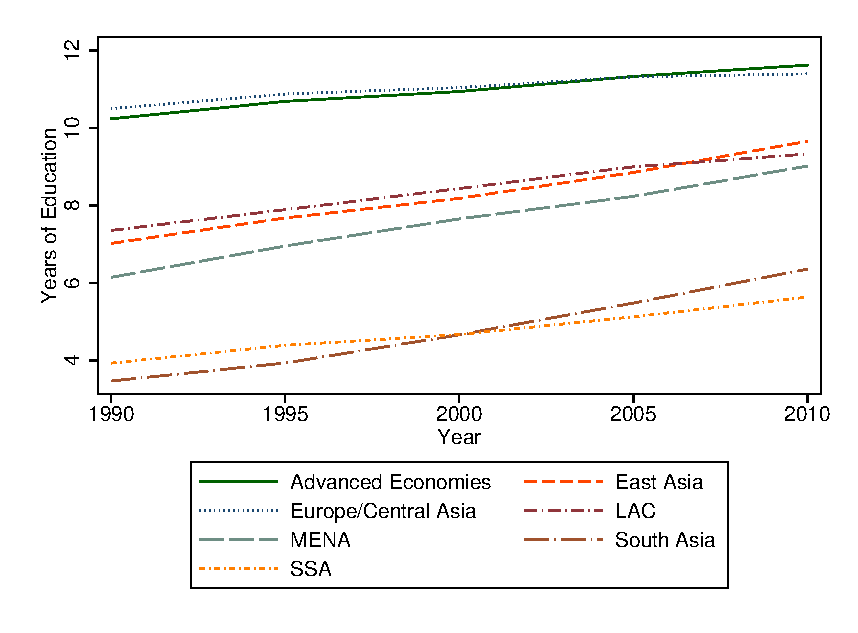
\includegraphics[scale=0.9]{\MMRfolder/Results/graphs/trends/SchoolingRegion.eps} 
\end{center}
\end{figure}

\begin{figure}[h!]
\begin{center}
\caption{Maternal Mortality Ratio by Region: 1990-2010}
\label{fig:MMRRegion}
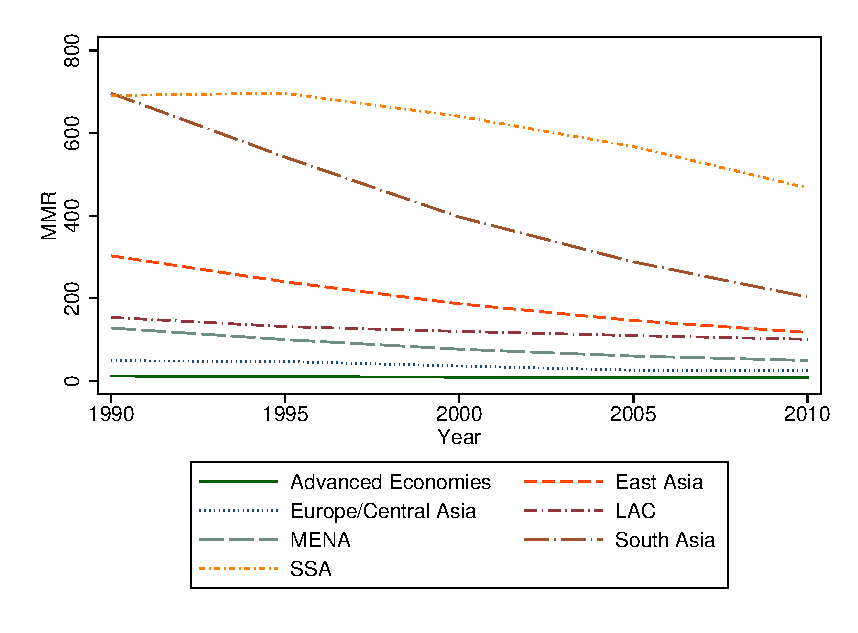
\includegraphics[scale=0.9]{\MMRfolder/Results/graphs/trends/MMRRegion.eps} 
\end{center}
\end{figure}

\begin{figure}[h!]
\begin{center}
\caption{Maternal Mortality and Education: Functional Form}
\label{fig:educmmr}
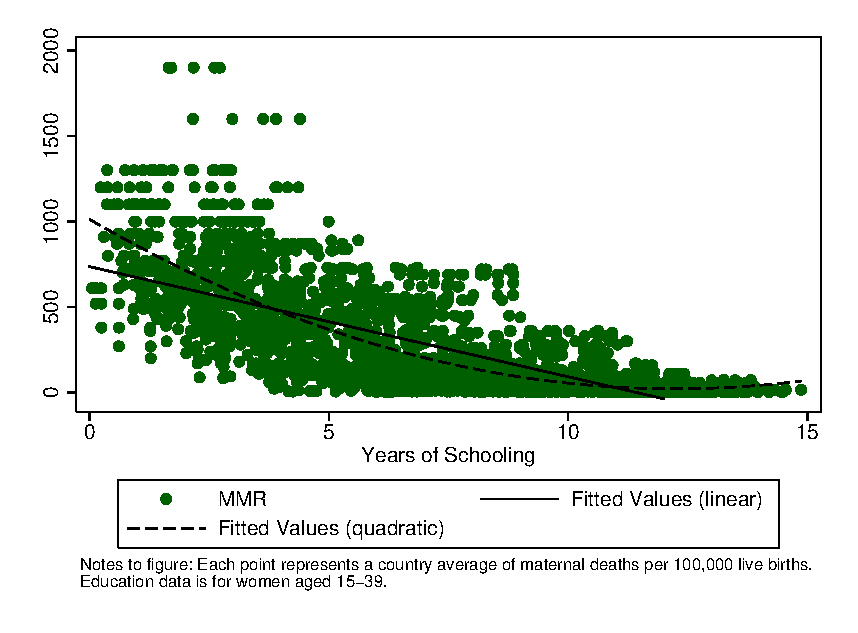
\includegraphics[scale=0.9]{\MMRfolder/Results/graphs/trends/Schooling_MMR_F.eps} 
\end{center}
\end{figure}

\begin{figure}[h!]
\begin{center}
\caption{Between and Within Country Correlations: Education and MMR}
\label{fig:arrows}
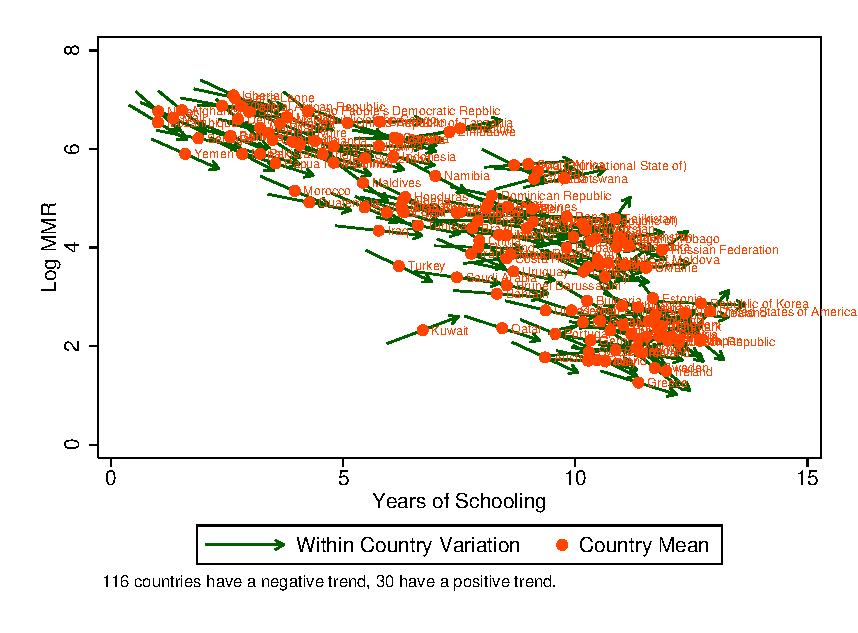
\includegraphics[scale=0.9]{\MMRfolder/Results/graphs/countries.eps} 
\end{center}
\end{figure}


\begin{landscape}
\begin{figure}[h!]
\begin{center}
\caption{Maternal Mortality Ratio by Country}
\label{fig:MMRGlobal}
\includegraphics[scale=0.9]{\MMRfolder/Results_aug2013/Graphs/MMR_2010.eps} 
\end{center}
\end{figure}
\end{landscape}


\begin{subfigures}
\begin{figure}[h!]
\begin{center}
\caption{Educational Attainment by Year -- Nigeria}
\label{fig:Nigeriaeduc}
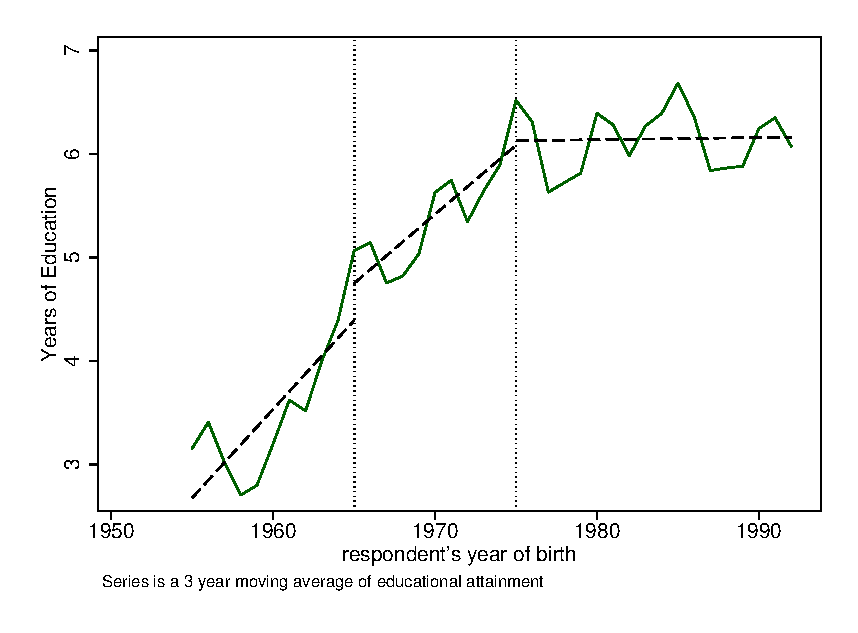
\includegraphics[scale=0.85]{\MMRfolder/Results/graphs/Nigeria_educ.eps} 
\end{center}
\end{figure}

\begin{figure}[h!]
\begin{center}
\caption{Maternal Mortality by Year -- Nigeria}
\label{fig:Nigeriammr}
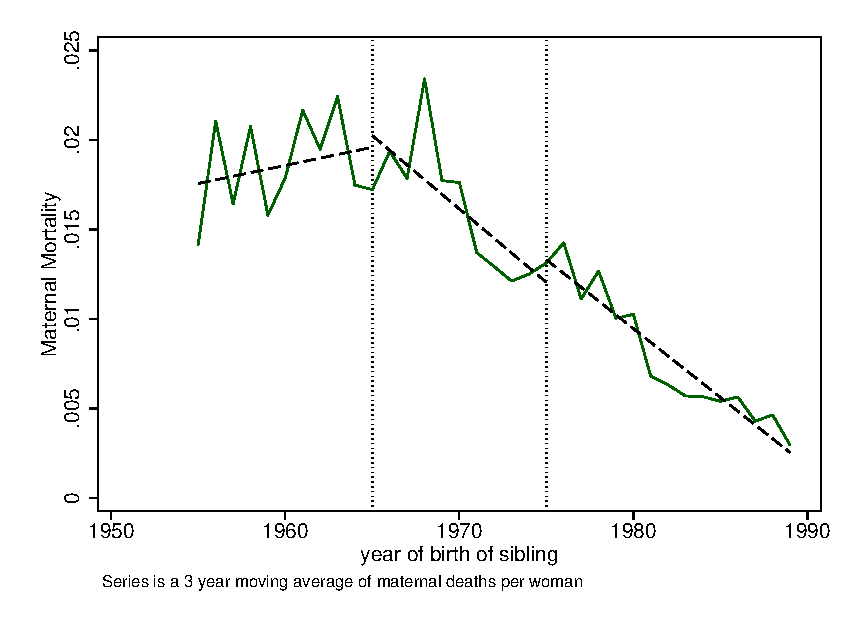
\includegraphics[scale=0.85]{\MMRfolder/Results/graphs/Nigeria_mmr.eps} 
\end{center}
\floatfoot{Note to figures \ref{fig:Nigeriaeduc}-\ref{fig:Nigeriammr}: 3 year moving
averages are displayed for maternal mortality and education.  The first vertical
dotted line represents the end of the control group, and the second vertical dotted
line represents the beginning of fully treated cohorts. Cohorts in between are
partially treated.  Further details in the body of the text, and table 
\ref{MMRtab:EducExp}.}
\end{figure}
\end{subfigures}

\clearpage

\begin{subfigures}
\begin{figure}[h!]
\begin{center}
\caption{Educational Attainment by Year -- Kenya}
\label{fig:Kenyaaeduc}
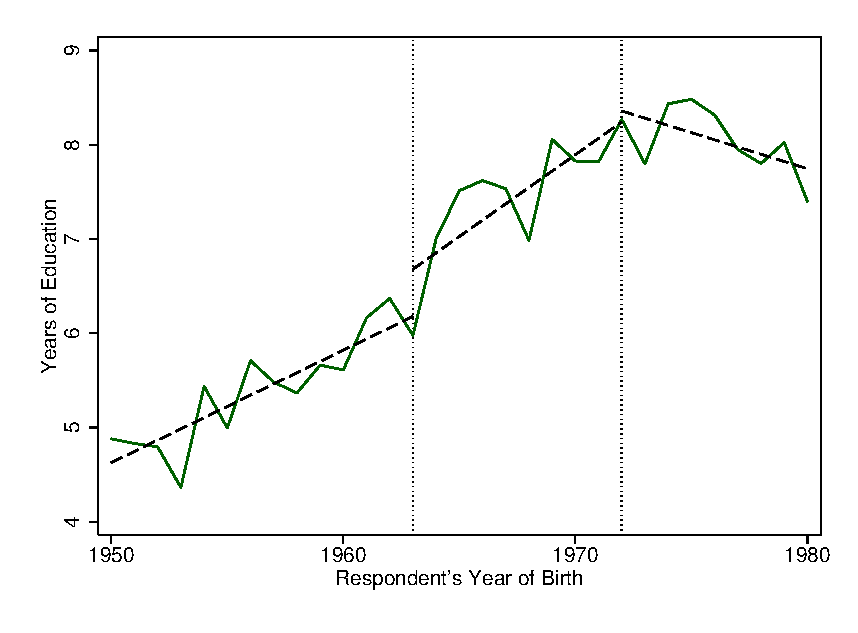
\includegraphics[scale=0.85]{\MMRfolder/Results/graphs/Kenya_educ.eps} 
\end{center}
\end{figure}

\begin{figure}[h!]
\begin{center}
\caption{Maternal Mortality by Year -- Kenya}
\label{fig:Kenyammr}
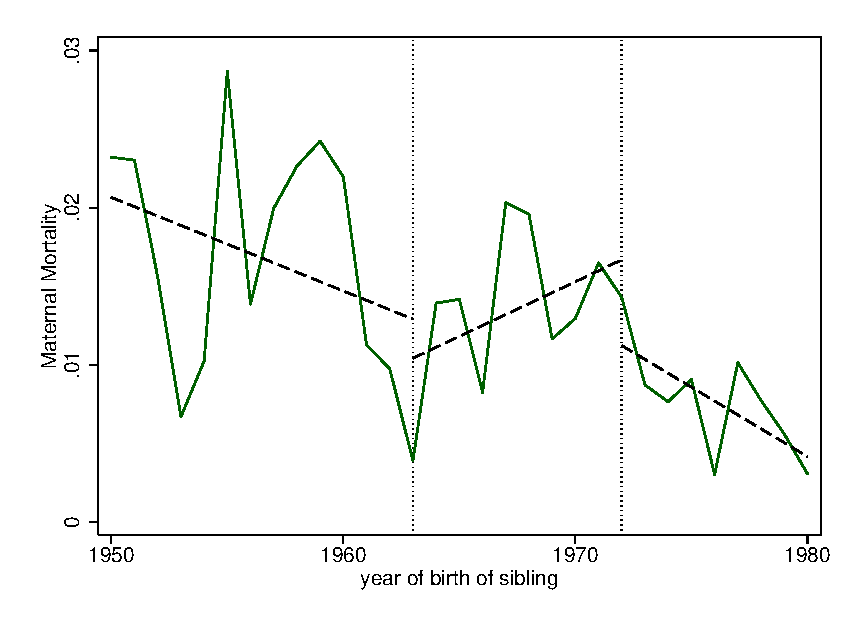
\includegraphics[scale=0.85]{\MMRfolder/Results/graphs/Kenya_mmr.eps} 
\end{center}
\floatfoot{Note to figures \ref{fig:Kenyaaeduc}-\ref{fig:Kenyammr}: The first 
vertical dotted line represents the end of the control group, and the second 
vertical dotted line represents the beginning of fully treated cohorts. Cohorts 
in between are partially treated.  Further details are provided in the body of 
the text, and in table \ref{MMRtab:EducExp}.}
\end{figure}
\end{subfigures}

\clearpage

\begin{subfigures}
\begin{figure}[h!]
\begin{center}
\caption{Educational Attainment by Year -- Zimbabwe}
\label{fig:Zimbabweeduc}
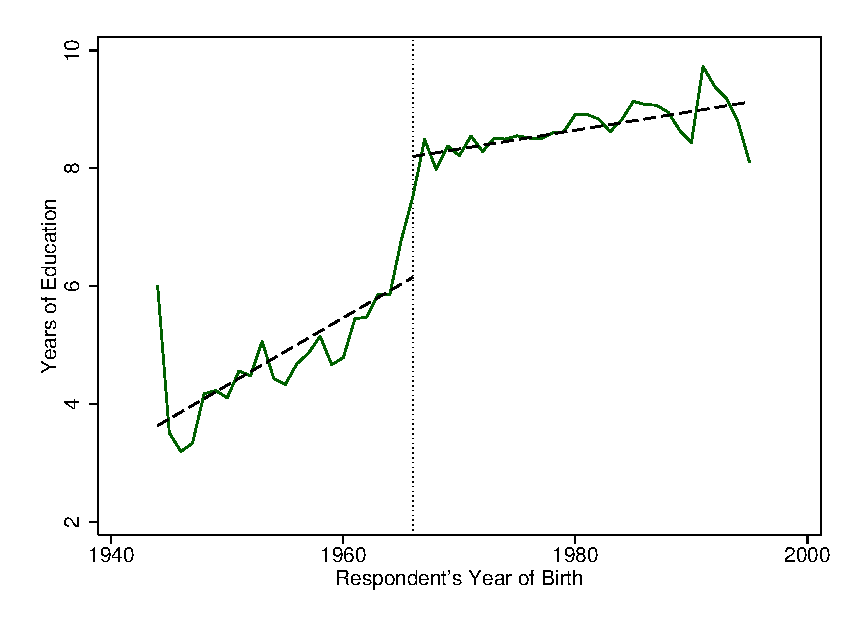
\includegraphics[scale=0.85]{\MMRfolder/Results/graphs/Zimbabwe_educ.eps} 
\end{center}
\end{figure}

\begin{figure}[h!]
\begin{center}
\caption{Maternal Mortality by Year -- Zimbabwe}
\label{fig:Zimbabwemmr}
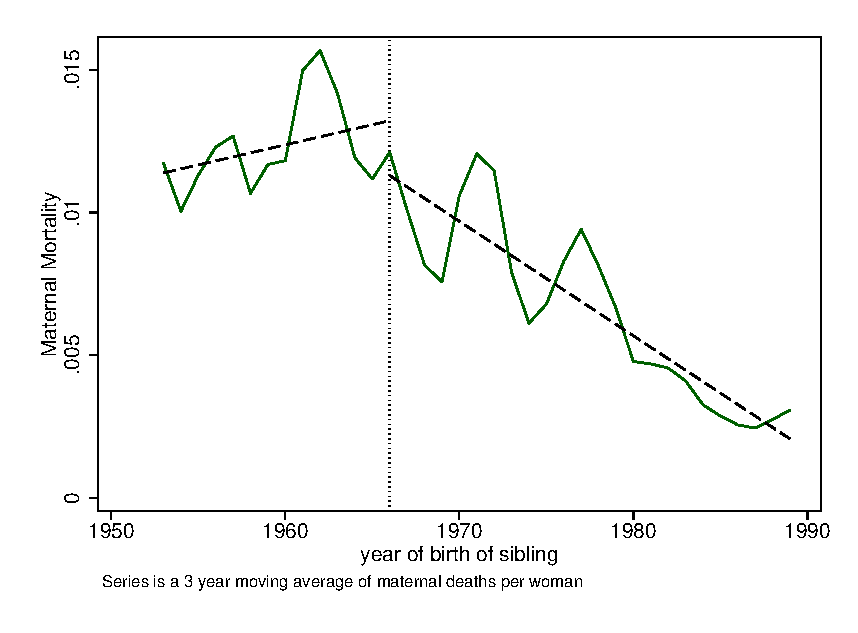
\includegraphics[scale=0.85]{\MMRfolder/Results/graphs/Zimbabwe_mmr.eps} 
\end{center}
\floatfoot{Note to figures \ref{fig:Zimbabweeduc}-\ref{fig:Zimbabwemmr}: 
Treatment was a one year expansion in schooling, differentially affecting
\emph{only} the 1965/1966 cohorts.  All cohorts to the left of the vertical
dotted line (1966 and after) are considered treated, and all cohorts to the 
right of the line (1965 and before) are not treated. Further details are 
provided in the body of the text, and in table \ref{MMRtab:EducExp}.}
\end{figure}
\end{subfigures}

\clearpage


\section*{Tables}
\begin{table}[htpb]
\begin{center}
\caption{Educational Experiments: treatment and control groups}
\label{MMRtab:EducExp}
\begin{tabular}{lclcc}
\toprule
Country & Year & Expansion & Treatment Years & Control Years \\ 
\midrule
Indonesia & 1973-78 & Primary school construction & 1968-72 & 1957-62  \\
Nigeria & 1976 & Universal Primary Education & 1970-75 & 1956-61 \\
Zimbabwe & 1980 & High school education expansion & 1966 & 1965 \\
Kenya & 1985 & Additional year of primary school & post-1972 & pre-1963 \\
Botswana & 1986 & High school year rearrangement & pre-1970, post 1982  & 1974 \\
Sierra Leone & 2001 & Free Primary Education & 1990-93 & 1980-86 \\
\bottomrule
\end{tabular}
\end{center}
\end{table}

\begin{subtables}
\begin{table}[htpb!]\begin{center}
\caption{Summary Statistics - Cross Country}\label{MMRtab:sumstats}
\begin{tabular}{lccccc}
&&&&& \\ \toprule Variable&Obs&Mean&Std. Dev.&Min&Max\\\midrule 
Maternal Mortality&710.0&220.6&300.9&2.0&1900.0\\
ln(Maternal Mortality)&710.0&4.302&1.649&0.6931&7.55\\
GDP per capita&702.0&9190.0&13870.0&64.36&104500.0\\
ln(GDP per capita)&702.0&7.966&1.649&4.164&11.56\\
Immunization&690.0&84.75&15.9&18.0&99.0\\
Fertility&718.0&3.163&1.676&0.887&8.659\\
Percent Attended Births&450.0&77.29&27.59&-2.6e-06&100.0\\
Population (Millions) &670.0&40.49&144.0&0.09515&1338.0\\
Teen Births&670.0&55.68&46.12&2.796&220.6\\
Husband wants more kids than wife&290.0&0.2107&0.07437&0.05331&0.3843\\
Husband wants less kids than wife&290.0&0.07031&0.03495&0.01606&0.1858\\
\midrule\multicolumn{6}{l}{\textsc{Education - Female}} \\ 
 Total Years of Education&730.0&8.07&3.319&0.4692&13.99\\
Years of Primary Education&730.0&4.714&1.693&0.3421&8.907\\
Years of Secondary Education&730.0&2.963&1.754&0.04875&7.459\\
Years of Tertiary Education&730.0&0.3932&0.3744&7.15e-08&2.048\\
Percent Primary&730.0&23.83&17.44&0.02&77.85\\
Percent Secondary&730.0&45.97&23.88&1.203&95.65\\
Percent Tertiary&730.0&12.58&12.05&0.0&62.86\\
Percent No Education&730.0&17.61&23.4&0.0&93.59\\
Male/Female Education (years)&730.0&1.16&0.4165&0.7114&4.499\\
\midrule
\multicolumn{6}{p{13.4cm}}{\begin{footnotesize}\textsc{Notes:} Maternal mortality is expressed in terms of    deaths per 100,000 live births. Immunization is expressed as the percent of   children of ages 12-23 months who are immunized against diphtheria, pertussis  and tetanus (DPT). Fertility represents births per woman, and teen births are expressed as the number of births per 1000 women between the ages of 15--19. Husband and wife fertility preferences are only available for DHS countries.\end{footnotesize}} \\ \bottomrule \end{tabular}\end{center}\end{table}
%\end{subtables}


\begin{table}[htpb!]											
\begin{center}											
\caption{Summary Statistics – Natural Experiments}											
\label{MMRtab:sumstatsexperiment}											
\begin{tabular}{l c c c c c}											
& & & & & \\											
\toprule											
Variable	&	Obs	&	Mean	&	Std. Dev.	&	Min	&	Max	\\
\midrule
\multicolumn{6}{l}{\textsc{Panel A – Nigeria}}  \\											
Years of Education	&	13221	&	4.822	&	5.349	&	0	&	22	\\
Investment per Capita	&	12748	&	0.881	&	0.545	&	0.014	&	2.195	\\
Non-West State	&	13235	&	0.828	&	0.377	&	0	&	1	\\
Year of Birth (education)	&	13235	&	1968.329	&	5.119	&	1956	&	1975	\\
Maternal Mortality	&	25354	&	0.019	&	0.137	&	0	&	1	\\
Under 25 Maternal Mortality	&	29676	&	0.006	&	0.074	&	0	&	1	\\
Year of Birth (MM)	&	29967	&	1968.472	&	5.381	&	1956	&	1975	\\
\midrule											
\multicolumn{6}{l}{\textsc{Panel B – Zimbabwe}}  \\											
Years of Education	&	10195	&	7.023	&	3.788	&	0	&	21	\\
High School Enrollment	&	10195	&	0.439	&	0.496	&	0	&	1	\\
Treated	&	10201	&	0.622	&	0.485	&	0	&	1	\\
Year of Birth (education)	&	10201	&	1966.128	&	4.786	&	1956	&	1974	\\
Maternal Mortality	&	23699	&	0.013	&	0.115	&	0	&	1	\\
Under 25 Maternal Mortality	&	28631	&	0.003	&	0.055	&	0	&	1	\\
Year of Birth (MM)	&	28842	&	1966.023	&	4.736	&	1957	&	1974	\\
\midrule											
\multicolumn{6}{l}{\textsc{Panel C – Kenya}}  \\											
Years of Education	&	13712	&	7.168	&	4.149	&	0	&	23	\\
Treated	&	13712	&	0.575	&	0.443	&	0	&	1	\\
Year of Birth (education)	&	13712	&	1968.389	&	8.147	&	1950	&	1980	\\
Maternal Mortality	&	22738	&	0.014	&	0.116	&	0	&	1	\\
Under 25 Maternal Mortality	&	25616	&	0.006	&	0.076	&	0	&	1	\\
Year of Birth (MM)	&	25686	&	1967.686	&	7.770	&	1950	&	1980	\\
\midrule											
\multicolumn{6}{p{12cm}}{\begin{footnotesize}\textsc{Notes:}  Year of birth (education) refers to the birth cohorts of respondents to the DHS surveys for whom we observe educational attainment.  Year of birth (MM) refers to the birth cohorts in the maternal mortality data, who are sisters of DHS respondents.  In panel A investment per capita refers to federal funds dispersed for school construction in 1976 (in naira).  We do not observe this for the state Abuja which has existed since 1991 only.  In all panels maternal mortality and under 25 maternal mortality refers deaths due to pregnancy divided by the total number of women. \end{footnotesize}} \\											
\bottomrule											
\end{tabular}											
\end{center}											
\end{table}											
\end{subtables}





\begin{landscape}\begin{table}[htpb!]\begin{center}\caption{Cross-Country Results of MMR and Female Educational Attainment}\label{MMRtab:MMRpercent}\begin{tabular}{lcccccccc}\toprule&\begin{footnotesize}(1)\end{footnotesize}&\begin{footnotesize}(2)\end{footnotesize}&\begin{footnotesize}(3)\end{footnotesize}&\begin{footnotesize}(4)\end{footnotesize}&\begin{footnotesize}(5)\end{footnotesize}&\begin{footnotesize}(6)\end{footnotesize}&\begin{footnotesize}(7)\end{footnotesize}&\begin{footnotesize}(8) \end{footnotesize}\\
VARIABLES&MMR&MMR&MMR&MMR&MMR&MMR&MMR&MMR\\ \midrule
&&&&&&&&\\
Primary Education (\% Population) &-10.06***&-10.24***&-8.463***&-8.445***&-7.738***&-7.386***&-7.185***&-6.597***\\
&\begin{footnotesize}(1.407)\end{footnotesize}&\begin{footnotesize}(1.625)\end{footnotesize}&\begin{footnotesize}(1.556)\end{footnotesize}&\begin{footnotesize}(1.559)\end{footnotesize}&\begin{footnotesize}(1.641)\end{footnotesize}&\begin{footnotesize}(1.710)\end{footnotesize}&\begin{footnotesize}(2.068)\end{footnotesize}&\begin{footnotesize}(1.941)\end{footnotesize}\\
Secondary Education (\% Population) &-9.696***&-9.789***&-6.672***&-6.689***&-5.979***&-5.375***&-5.146***&-4.514***\\
&\begin{footnotesize}(1.214)\end{footnotesize}&\begin{footnotesize}(1.305)\end{footnotesize}&\begin{footnotesize}(1.376)\end{footnotesize}&\begin{footnotesize}(1.367)\end{footnotesize}&\begin{footnotesize}(1.432)\end{footnotesize}&\begin{footnotesize}(1.578)\end{footnotesize}&\begin{footnotesize}(1.872)\end{footnotesize}&\begin{footnotesize}(1.716)\end{footnotesize}\\
Tertiary Education (\% Population) &-9.521***&-10.35***&-4.618**&-4.741**&-4.501**&-4.126**&-4.061**&-3.651**\\
&\begin{footnotesize}(1.238)\end{footnotesize}&\begin{footnotesize}(1.412)\end{footnotesize}&\begin{footnotesize}(2.035)\end{footnotesize}&\begin{footnotesize}(1.968)\end{footnotesize}&\begin{footnotesize}(1.854)\end{footnotesize}&\begin{footnotesize}(1.928)\end{footnotesize}&\begin{footnotesize}(1.965)\end{footnotesize}&\begin{footnotesize}(1.833)\end{footnotesize}\\
year 1995&&&-11.36&-12.13&-4.635&-4.217&-2.281&-7.504\\
&&&\begin{footnotesize}(12.82)\end{footnotesize}&\begin{footnotesize}(13.39)\end{footnotesize}&\begin{footnotesize}(12.28)\end{footnotesize}&\begin{footnotesize}(11.90)\end{footnotesize}&\begin{footnotesize}(14.28)\end{footnotesize}&\begin{footnotesize}(14.95)\end{footnotesize}\\
year 2000&&&-30.15*&-31.06*&-19.39&-16.87&-13.19&-16.39\\
&&&\begin{footnotesize}(17.38)\end{footnotesize}&\begin{footnotesize}(18.21)\end{footnotesize}&\begin{footnotesize}(16.56)\end{footnotesize}&\begin{footnotesize}(16.27)\end{footnotesize}&\begin{footnotesize}(21.04)\end{footnotesize}&\begin{footnotesize}(21.15)\end{footnotesize}\\
year 2005&&&-56.27**&-60.50**&-37.83&-37.68&-32.58&-28.84\\
&&&\begin{footnotesize}(22.49)\end{footnotesize}&\begin{footnotesize}(27.52)\end{footnotesize}&\begin{footnotesize}(24.31)\end{footnotesize}&\begin{footnotesize}(23.39)\end{footnotesize}&\begin{footnotesize}(29.22)\end{footnotesize}&\begin{footnotesize}(28.47)\end{footnotesize}\\
year 2010&&&-80.21***&-87.56**&-63.80*&-62.16*&-56.23&-42.41\\
&&&\begin{footnotesize}(27.81)\end{footnotesize}&\begin{footnotesize}(38.27)\end{footnotesize}&\begin{footnotesize}(33.73)\end{footnotesize}&\begin{footnotesize}(32.62)\end{footnotesize}&\begin{footnotesize}(38.68)\end{footnotesize}&\begin{footnotesize}(37.38)\end{footnotesize}\\
log GDP per capita&&&&8.223&5.817&9.654&8.563&5.675\\
&&&&\begin{footnotesize}(20.83)\end{footnotesize}&\begin{footnotesize}(20.45)\end{footnotesize}&\begin{footnotesize}(20.13)\end{footnotesize}&\begin{footnotesize}(19.69)\end{footnotesize}&\begin{footnotesize}(19.57)\end{footnotesize}\\
Immunization (DPT) &&&&&-2.194**&-2.022**&-1.978**&-1.950**\\
&&&&&\begin{footnotesize}(0.886)\end{footnotesize}&\begin{footnotesize}(0.880)\end{footnotesize}&\begin{footnotesize}(0.909)\end{footnotesize}&\begin{footnotesize}(0.913)\end{footnotesize}\\
Attended Births&&&&&&-1.275&-1.172&-1.451*\\
&&&&&&\begin{footnotesize}(0.813)\end{footnotesize}&\begin{footnotesize}(0.791)\end{footnotesize}&\begin{footnotesize}(0.804)\end{footnotesize}\\
Fertility&&&&&&&8.339&-5.573\\
&&&&&&&\begin{footnotesize}(25.38)\end{footnotesize}&\begin{footnotesize}(25.92)\end{footnotesize}\\
Teen births&&&&&&&&1.835**\\
&&&&&&&&\begin{footnotesize}(0.908)\end{footnotesize}\\
Constant&1,022***&1,044***&824.6***&764.7***&904.4***&915.6***&866.4***&795.2***\\
&\begin{footnotesize}(100.4)\end{footnotesize}&\begin{footnotesize}(113.8)\end{footnotesize}&\begin{footnotesize}(114.1)\end{footnotesize}&\begin{footnotesize}(205.4)\end{footnotesize}&\begin{footnotesize}(200.9)\end{footnotesize}&\begin{footnotesize}(191.9)\end{footnotesize}&\begin{footnotesize}(277.4)\end{footnotesize}&\begin{footnotesize}(289.2)\end{footnotesize}\\
&&&&&&&&\\
Observations&710&428&428&428&428&428&428&428\\
R-squared&0.344&0.450&0.489&0.490&0.519&0.529&0.529&0.542\\
Number of countries&142&108&108&108&108&108&108&108\\
\midrule
\multicolumn{9}{p{20cm}}{\begin{footnotesize}\textsc{Notes:} All regressions include fixed-effects by country. For the full list of countries by year see online appendix table 1.  Results are for the percent of the female population between the ages of  15 and 39 with each level of education in each country.  A full description of control variables is available in section \ref{scn:data}, and as the note to table \ref{MMRtab:sumstats}.  Standard errors clustered at the level of the country are diplayed.
$^{*}$p$<$0.1; $^{**}$p$<$0.05; $^{***}$p$<$0.01\end{footnotesize}} \\ \bottomrule 
\end{tabular}\end{center}\end{table}\end{landscape}

\begin{subtables}\begin{landscape}\begin{table}[htpb!]\begin{center}\caption{Cross-Country Results of MMR and Female Educational Attainment By Region}\label{MMRtab:MMRregion}\begin{tabular}{lccccccc}\toprule&(1)&(2)&(3)&(4)&(5)&(6)&(7)\\&Advanced&East Asia&Europe and&Latin Amer-&Middle East&South&Sub-Saharan\\VARIABLES&Economies&and the&Central &ica and the&and North&Asia&Africa\\&&Pacific&Asia&Caribbean&Africa&&\\ \midrule 
 \vspace{4pt}&\begin{footnotesize}\end{footnotesize}&\begin{footnotesize}\end{footnotesize}&\begin{footnotesize}\end{footnotesize}&\begin{footnotesize}\end{footnotesize}&\begin{footnotesize}\end{footnotesize}&\begin{footnotesize}\end{footnotesize}&\begin{footnotesize}\end{footnotesize}\\Primary Education (\% Population) &-1.117*&-8.910**&3.508*&-5.732**&0.0997&-8.119*&-10.43**\\
&\begin{footnotesize}(0.537)\end{footnotesize}&\begin{footnotesize}(2.890)\end{footnotesize}&\begin{footnotesize}(1.771)\end{footnotesize}&\begin{footnotesize}(2.706)\end{footnotesize}&\begin{footnotesize}(0.902)\end{footnotesize}&\begin{footnotesize}(3.909)\end{footnotesize}&\begin{footnotesize}(4.206)\end{footnotesize}\\
Secondary Education (\% Population) &-1.077*&-7.771**&4.355*&-4.173&-0.487&-12.20&-2.061\\
&\begin{footnotesize}(0.525)\end{footnotesize}&\begin{footnotesize}(2.847)\end{footnotesize}&\begin{footnotesize}(2.226)\end{footnotesize}&\begin{footnotesize}(2.456)\end{footnotesize}&\begin{footnotesize}(1.337)\end{footnotesize}&\begin{footnotesize}(7.065)\end{footnotesize}&\begin{footnotesize}(5.725)\end{footnotesize}\\
Tertiary Education (\% Population) &-0.704&-2.574&5.997**&-5.795**&-2.735**&14.49&1.311\\
&\begin{footnotesize}(0.498)\end{footnotesize}&\begin{footnotesize}(5.957)\end{footnotesize}&\begin{footnotesize}(2.785)\end{footnotesize}&\begin{footnotesize}(2.701)\end{footnotesize}&\begin{footnotesize}(1.188)\end{footnotesize}&\begin{footnotesize}(24.04)\end{footnotesize}&\begin{footnotesize}(19.45)\end{footnotesize}\\
Constant&110.9**&901.1***&-364.6*&614.4**&160.1**&945.6***&1,087***\\
&\begin{footnotesize}(50.11)\end{footnotesize}&\begin{footnotesize}(231.4)\end{footnotesize}&\begin{footnotesize}(199.5)\end{footnotesize}&\begin{footnotesize}(227.1)\end{footnotesize}&\begin{footnotesize}(54.94)\end{footnotesize}&\begin{footnotesize}(179.4)\end{footnotesize}&\begin{footnotesize}(235.2)\end{footnotesize}\\
&&&&&&&\\
Observations&78&42&67&83&34&23&101\\
R-squared&0.554&0.682&0.540&0.503&0.590&0.935&0.607\\
Number of countries&18&11&16&20&12&6&25\\
\midrule
\multicolumn{8}{p{20cm}}{\begin{footnotesize}\textsc{Notes:} All regressions include fixed-effects by country.  Results are for average years of education of females between the ages of 15 and 39 in each country.  Results are reported for specification (2) from table \ref{MMRtab:MMRpercent} which includes country and year fixed effects.  Standard errors are clustered by country.
$^{*}$p$<$0.1; $^{**}$p$<$0.05; $^{***}$p$<$0.01\end{footnotesize}} \\ \bottomrule 
\end{tabular}\end{center}\end{table}\end{landscape}
\begin{table}[htpb!]\begin{center}\caption{Cross-Country Results of MMR and Female Educational Attainment By Income Group}\label{MMRtab:MMRincome}\begin{tabular}{lcccc}\toprule 
 &(1)&(2)&(3)&(4)\\VARIABLES&Low&Lower&Upper&High\\&&Middle&Middle&\\ \midrule
 \vspace{4pt}&\begin{footnotesize}\end{footnotesize}&\begin{footnotesize}\end{footnotesize}&\begin{footnotesize}\end{footnotesize}&\begin{footnotesize}\end{footnotesize}\\Primary Education (\% Population) &-9.972*&-5.157**&-3.567&0.0519\\
&\begin{footnotesize}(4.759)\end{footnotesize}&\begin{footnotesize}(2.210)\end{footnotesize}&\begin{footnotesize}(2.306)\end{footnotesize}&\begin{footnotesize}(0.0779)\end{footnotesize}\\
Secondary Education (\% Population) &-0.877&-5.469**&-2.743&-0.0237\\
&\begin{footnotesize}(5.349)\end{footnotesize}&\begin{footnotesize}(2.350)\end{footnotesize}&\begin{footnotesize}(2.330)\end{footnotesize}&\begin{footnotesize}(0.104)\end{footnotesize}\\
Tertiary Education (\% Population) &-8.746&-10.18**&-2.362&0.0860\\
&\begin{footnotesize}(36.03)\end{footnotesize}&\begin{footnotesize}(4.340)\end{footnotesize}&\begin{footnotesize}(1.978)\end{footnotesize}&\begin{footnotesize}(0.147)\end{footnotesize}\\
Constant&1,097***&781.4***&373.3*&12.43\\
&\begin{footnotesize}(178.4)\end{footnotesize}&\begin{footnotesize}(167.3)\end{footnotesize}&\begin{footnotesize}(200.3)\end{footnotesize}&\begin{footnotesize}(9.365)\end{footnotesize}\\
&&&&\\
Observations&79&114&122&113\\
R-squared&0.769&0.540&0.349&0.124\\
Number of countries&19&28&31&30\\
\midrule
\multicolumn{5}{p{12.5cm}}{\begin{footnotesize}\textsc{Notes:} All regressions include fixed-effects by country.  Results are for average years of education of females between the ages of 15 and 39 in each country.  Results are reported for specification (2) from table \ref{MMRtab:MMRpercent} which includes country and year fixed effects.  Countries are classified according to World Bank income groups, and standard errors are clustered by country.
$^{*}$p$<$0.1; $^{**}$p$<$0.05; $^{***}$p$<$0.01\end{footnotesize}} \\ \bottomrule 
\end{tabular}\end{center}\end{table}\end{subtables}
\begin{landscape}\begin{table}[htpb!]\begin{center}\caption{Cross-Country Results: MMR and Female versus Male Education}\label{MMRtab:MMRgender}\begin{tabular}{lcccccccc}\toprule&\begin{footnotesize}(1)\end{footnotesize}&\begin{footnotesize}(2)\end{footnotesize}&\begin{footnotesize}(3)\end{footnotesize}&\begin{footnotesize}(4)\end{footnotesize}&\begin{footnotesize}(5)\end{footnotesize}&\begin{footnotesize}(6)\end{footnotesize}&\begin{footnotesize}(7)\end{footnotesize}&\begin{footnotesize}(8) \end{footnotesize}\\
VARIABLES&MMR&MMR&MMR&MMR&MMR&MMR&MMR&MMR\\ \midrule
&&&&&&&&\\
Primary Education (\% Females) &-13.41***&-16.37***&-14.41***&-14.34***&-13.42***&-11.97***&-12.10***&-11.18**\\
&\begin{footnotesize}(2.576)\end{footnotesize}&\begin{footnotesize}(4.528)\end{footnotesize}&\begin{footnotesize}(4.311)\end{footnotesize}&\begin{footnotesize}(4.326)\end{footnotesize}&\begin{footnotesize}(4.310)\end{footnotesize}&\begin{footnotesize}(4.270)\end{footnotesize}&\begin{footnotesize}(4.348)\end{footnotesize}&\begin{footnotesize}(4.357)\end{footnotesize}\\
Secondary Education (\% Females) &-8.008***&-13.38***&-8.637**&-8.642**&-7.538**&-6.686*&-6.951*&-6.420*\\
&\begin{footnotesize}(2.402)\end{footnotesize}&\begin{footnotesize}(3.778)\end{footnotesize}&\begin{footnotesize}(3.980)\end{footnotesize}&\begin{footnotesize}(3.968)\end{footnotesize}&\begin{footnotesize}(3.692)\end{footnotesize}&\begin{footnotesize}(3.728)\end{footnotesize}&\begin{footnotesize}(3.740)\end{footnotesize}&\begin{footnotesize}(3.605)\end{footnotesize}\\
Tertiary Education (\% Females) &-7.481***&-10.69**&-0.0648&-0.145&-0.1000&0.289&0.231&0.171\\
&\begin{footnotesize}(2.648)\end{footnotesize}&\begin{footnotesize}(4.151)\end{footnotesize}&\begin{footnotesize}(6.655)\end{footnotesize}&\begin{footnotesize}(6.525)\end{footnotesize}&\begin{footnotesize}(5.774)\end{footnotesize}&\begin{footnotesize}(5.894)\end{footnotesize}&\begin{footnotesize}(5.867)\end{footnotesize}&\begin{footnotesize}(5.719)\end{footnotesize}\\
Primary Education (\% Males) &3.674&8.955&8.946&8.819&8.649*&7.618&7.668&7.195\\
&\begin{footnotesize}(3.487)\end{footnotesize}&\begin{footnotesize}(6.055)\end{footnotesize}&\begin{footnotesize}(5.511)\end{footnotesize}&\begin{footnotesize}(5.509)\end{footnotesize}&\begin{footnotesize}(5.199)\end{footnotesize}&\begin{footnotesize}(5.016)\end{footnotesize}&\begin{footnotesize}(5.027)\end{footnotesize}&\begin{footnotesize}(5.054)\end{footnotesize}\\
Secondary Education (\% Males) &-2.006&6.088&5.040&4.943&4.411&4.458&4.601&4.510\\
&\begin{footnotesize}(3.528)\end{footnotesize}&\begin{footnotesize}(5.270)\end{footnotesize}&\begin{footnotesize}(4.741)\end{footnotesize}&\begin{footnotesize}(4.766)\end{footnotesize}&\begin{footnotesize}(4.242)\end{footnotesize}&\begin{footnotesize}(4.230)\end{footnotesize}&\begin{footnotesize}(4.221)\end{footnotesize}&\begin{footnotesize}(4.198)\end{footnotesize}\\
Tertiary Education (\% Males) &-2.993&0.781&-3.526&-3.808&-3.570&-3.299&-3.287&-2.903\\
&\begin{footnotesize}(3.985)\end{footnotesize}&\begin{footnotesize}(5.931)\end{footnotesize}&\begin{footnotesize}(6.879)\end{footnotesize}&\begin{footnotesize}(6.897)\end{footnotesize}&\begin{footnotesize}(6.075)\end{footnotesize}&\begin{footnotesize}(6.152)\end{footnotesize}&\begin{footnotesize}(6.168)\end{footnotesize}&\begin{footnotesize}(6.086)\end{footnotesize}\\
&&&&&&&&\\Observations&710&428&428&428&428&428&428&428\\
R-squared&0.560&0.610&0.655&0.656&0.682&0.691&0.692&0.696\\
Number of countries&142&108&108&108&108&108&108&108\\
\midrule
\multicolumn{9}{p{20cm}}{\begin{footnotesize}\textsc{Notes:} All regressions include fixed-effects by country. For the full list of countries by year see online appendix table 1. Educational variables are the same as those in table \ref{MMRtab:MMRpercent} however include both female and male figures for each variable (ages 15-39). A full description of control variables is available in section \ref{scn:data}, and as the note to table \ref{MMRtab:sumstats}.  Standard errors clustered at the level of the country are diplayed.
$^{*}$p$<$0.1; $^{**}$p$<$0.05; $^{***}$p$<$0.01\end{footnotesize}} \\ \bottomrule 
\end{tabular}\end{center}\end{table}\end{landscape}


\begin{landscape}\begin{table}[htpb!]\begin{center}\caption{Correlations between Education and Health/Development Outcomes}\label{MMRtab:Zscore}\begin{tabular}{lccccc}\toprule 
 &(1)&(2)&(3)&(4)&(5)\\VARIABLES&Fertility&Immunization&Percent Attend&ln(GDP pc)& Teen Births\\\midrule
 \vspace{4pt}&\begin{footnotesize}\end{footnotesize}&\begin{footnotesize}\end{footnotesize}&\begin{footnotesize}\end{footnotesize}&\begin{footnotesize}\end{footnotesize}&\begin{footnotesize}\end{footnotesize}\\Primary Education (\% Population) &-0.0177***&0.0147***&0.0138***&0.00793***&-0.00829***\\
&\begin{footnotesize}(0.00165)\end{footnotesize}&\begin{footnotesize}(0.00281)\end{footnotesize}&\begin{footnotesize}(0.00234)\end{footnotesize}&\begin{footnotesize}(0.00144)\end{footnotesize}&\begin{footnotesize}(0.00285)\end{footnotesize}\\
Secondary Education (\% Population) &-0.0315***&0.0261***&0.0315***&0.0181***&-0.0243***\\
&\begin{footnotesize}(0.00105)\end{footnotesize}&\begin{footnotesize}(0.00193)\end{footnotesize}&\begin{footnotesize}(0.00152)\end{footnotesize}&\begin{footnotesize}(0.00119)\end{footnotesize}&\begin{footnotesize}(0.00187)\end{footnotesize}\\
Tertiary Education (\% Population) &-0.0377***&0.0241***&0.0320***&0.0483***&-0.0293***\\
&\begin{footnotesize}(0.00161)\end{footnotesize}&\begin{footnotesize}(0.00237)\end{footnotesize}&\begin{footnotesize}(0.00296)\end{footnotesize}&\begin{footnotesize}(0.00273)\end{footnotesize}&\begin{footnotesize}(0.00223)\end{footnotesize}\\
Constant&2.331***&-1.836***&-2.193***&-1.629***&1.688***\\
&\begin{footnotesize}(0.0798)\end{footnotesize}&\begin{footnotesize}(0.180)\end{footnotesize}&\begin{footnotesize}(0.146)\end{footnotesize}&\begin{footnotesize}(0.0639)\end{footnotesize}&\begin{footnotesize}(0.174)\end{footnotesize}\\
&&&&\\
Observations&718&690&450&702&670\\
R-squared&0.723&0.417&0.692&0.581&0.482\\
\midrule
\multicolumn{6}{p{17.7cm}}{\begin{footnotesize}\textsc{Notes:} Each regression includes fixed effects by country, and heteroscedasticity robust standard errors.  Each dependent variable has been transformed to a z-score by subtracting its global mean and dividing by its standard deviation.  Education measures are for the female population between 15 and 39. For discussion of the effect size, see section \ref{ssscn:effects}.
$^{*}$p$<$0.1; $^{**}$p$<$0.05; $^{***}$p$<$0.01\end{footnotesize}} \\ \bottomrule 
\end{tabular}\end{center}\end{table}\end{landscape}

\begin{subtables}\begin{table}[htpb!]\begin{center}\caption{Effect of 1976 Educational Expansion: Nigeria}\label{MMRtab:Nigeria}\begin{tabular}{p{5cm}cccc}\toprule&(1)&(2)&(3)&(4)\\ \midrule\multicolumn{5}{l}{\textsc{Panel A: Outcome -- Education}}\\\begin{footnotesize}\end{footnotesize}&\begin{footnotesize}\end{footnotesize}&\begin{footnotesize}\end{footnotesize}&\begin{footnotesize}\end{footnotesize}\\ 
Intensity 70-75&0.983*&2.147***&0.0574&0.175***\\ 
&\begin{footnotesize}(0.555)\end{footnotesize}&\begin{footnotesize}(0.790)\end{footnotesize}&\begin{footnotesize}(0.0545)\end{footnotesize}&\begin{footnotesize}(0.0451)\end{footnotesize}\\ 
Intensity 65-69&0.671*&1.040**&0.0925&0.195***\\ 
&\begin{footnotesize}(0.382)\end{footnotesize}&\begin{footnotesize}(0.445)\end{footnotesize}&\begin{footnotesize}(0.0641)\end{footnotesize}&\begin{footnotesize}(0.0540)\end{footnotesize}\\ 
Intensity      &0.360&&&\\ 
&\begin{footnotesize}(0.513)\end{footnotesize}&&\\ 
\begin{footnotesize}\end{footnotesize}&\begin{footnotesize}\end{footnotesize}&\begin{footnotesize}\end{footnotesize}&\begin{footnotesize}\end{footnotesize}\\ 
Observations&12,735&12,735&12,735&12,735\\ 
R-squared&0.425&0.424&0.426&0.427\\ \midrule 
\multicolumn{5}{l}{\textsc{Panel B: Outcome -- MMR}}\\ 
\begin{footnotesize}\end{footnotesize}&\begin{footnotesize}\end{footnotesize}&\begin{footnotesize}\end{footnotesize}&\begin{footnotesize}\end{footnotesize}\\ 
Intensity 70-75&-0.000214&-0.0135&-2.67e-05&2.95e-05\\ 
&\begin{footnotesize}(0.00867)\end{footnotesize}&\begin{footnotesize}(0.0116)\end{footnotesize}&\begin{footnotesize}(0.000877)\end{footnotesize}&\begin{footnotesize}(0.000753)\end{footnotesize}\\ 
Intensity 65-69&-0.000119&-0.00839&0.00257*&0.00161\\ 
&\begin{footnotesize}(0.00637)\end{footnotesize}&\begin{footnotesize}(0.00752)\end{footnotesize}&\begin{footnotesize}(0.00153)\end{footnotesize}&\begin{footnotesize}(0.00121)\end{footnotesize}\\ 
Intensity      &0.000119&&&\\ 
&\begin{footnotesize}(0.00812)\end{footnotesize}&&\\ 
\begin{footnotesize}\end{footnotesize}&\begin{footnotesize}\end{footnotesize}&\begin{footnotesize}\end{footnotesize}&\begin{footnotesize}\end{footnotesize}\\ 
Observations&28,694&28,694&28,694&28,694\\ 
R-squared&0.008&0.008&0.013&0.013\\ \midrule 
\multicolumn{5}{l}{\textsc{Panel C: Outcome -- MMR (Under 25)}}\\ 
\begin{footnotesize}\end{footnotesize}&\begin{footnotesize}\end{footnotesize}&\begin{footnotesize}\end{footnotesize}&\begin{footnotesize}\end{footnotesize}\\ 
Intensity 70-75&-0.000323&-0.0192**&-0.00128*&-0.00120***\\ 
&\begin{footnotesize}(0.00546)\end{footnotesize}&\begin{footnotesize}(0.00949)\end{footnotesize}&\begin{footnotesize}(0.000650)\end{footnotesize}&\begin{footnotesize}(0.000336)\end{footnotesize}\\ 
Intensity 65-69&-0.00162&-0.0118**&-0.000768&-0.00151***\\ 
&\begin{footnotesize}(0.00353)\end{footnotesize}&\begin{footnotesize}(0.00517)\end{footnotesize}&\begin{footnotesize}(0.000712)\end{footnotesize}&\begin{footnotesize}(0.000500)\end{footnotesize}\\ 
Intensity      &-0.00419&&&\\ 
&\begin{footnotesize}(0.00513)\end{footnotesize}&&\\ 
\begin{footnotesize}\end{footnotesize}&\begin{footnotesize}\end{footnotesize}&\begin{footnotesize}\end{footnotesize}&\begin{footnotesize}\end{footnotesize}\\ 
Observations&28,694&28,694&28,694&28,694\\ 
R-squared&0.005&0.005&0.007&0.007\\ 
\midrule
\multicolumn{5}{p{12.7cm}}{\begin{footnotesize}\textsc{Notes:} Columns (1)-(4) represent different measures of treatment intensity. Column (1) uses capital expenditure on school construction in 1976 in each individual's state as their treatment intensity, column (2) uses a dummy for residence in non-West (high-intensity) states, column (3) uses the number of years exposed to the reform interacted with the high-intensity state dummy as the intensity measure, and column (4) uses capital expenditure interacted with the high-intensity state dummy.  The effect of the reform is identified for 1970-1975 birth cohorts (who are fully affected), and 1965-1969 cohorts, who are affected partially via over-age enrollments. Panel A shows the effect of the education reforms on educational attainment, panel B shows the effect on life-time maternal mortality, and panel C the effect on maternal mortality under the age of 25.  All regressions are double-differences, however in columns (2)-(4) the intensity dummy is captured by state of residence fixed effects. Additional controls include religion, ethnicity and year of birth fixed effects, plus time trends by state, and controls for the length of exposure to the civil war in Biafra \citep{Akreshetal2012}.  Standard errors are clustered by state and birth cohort.
$^{*}$p$<$0.1; $^{**}$p$<$0.05; $^{***}$p$<$0.01\end{footnotesize}} \\ \bottomrule 
\end{tabular}\end{center}\end{table}
\begin{landscape}\begin{table}[htpb!]\begin{center}
\caption{Effect of 1980 Educational Expansion: Zimbabwe}
\label{MMRtab:Zimbabwe}\begin{tabular}{lcccccc}\toprule
& \multicolumn{3}{c}{Years of Education}&\multicolumn{3}{c}{Maternal Mortality }\\VARIABLES & (1)&(2)&(3)&(4)&(5)&(6)\\ \cmidrule(r){1-4} \cmidrule(r){5-7}\begin{footnotesize}\end{footnotesize}&\begin{footnotesize}\end{footnotesize}&\begin{footnotesize}\end{footnotesize}&\begin{footnotesize}\end{footnotesize}&\begin{footnotesize}\end{footnotesize}&\begin{footnotesize}\end{footnotesize}\\ 
DumAge&1.244***&0.446**&0.509&-0.00413**&-0.000283&0.00265\\
&(0.196)&(0.182)&(0.327)&(0.00143)&(0.00451)&(0.00701)\\
DumAge$\times$(Age1980-14)&-0.186***&-0.575***&-0.934***&0.000155&0.000186&0.000582\\
&(0.0257)&(0.0682)&(0.189)&(0.000311)&(0.00107)&(0.00227)\\
(1-DumAge)$\times$(Age1980-14)&-0.135***&-0.324**&-0.0588&-0.000249&0.00219&0.00516\\
&(0.0313)&(0.113)&(0.299)&(0.000432)&(0.00235)&(0.00676)\\
\begin{footnotesize}\end{footnotesize}&\begin{footnotesize}\end{footnotesize}&\begin{footnotesize}\end{footnotesize}&\begin{footnotesize}\end{footnotesize}&\begin{footnotesize}\end{footnotesize}&\begin{footnotesize}\end{footnotesize}\\ 
Observations&10,198&10,198&10,198&28,631&28,631&28,631\\
R-squared&0.223&0.226&0.227&0.002&0.002&0.002\\
\midrule
\multicolumn{7}{p{15.4cm}}{\begin{footnotesize}\textsc{Notes:} Columns (1) and (4) include a linear trend for age, columns (2) and (5) a quadratic, and columns (3) and (6) a cubic trend.  DumAge (treatment) refers to the birth cohort which was 14 years old at the time of the reform (1980).  Additional controls included are survey, region and birth cohort fixed effects, along with a rural dummy variable. Standard errors are clustered at region of residence.
$^{*}$p$<$0.1; $^{**}$p$<$0.05; $^{***}$p$<$0.01\end{footnotesize}} \\ \bottomrule 
\end{tabular}\end{center}\end{table}\end{landscape}
\begin{table}[htpb!]\begin{center}\caption{Effect of 1985 Educational Expansion: Kenya}\label{MMRtab:Kenya}\begin{tabular}{p{3cm}cc}\toprule&(1)&(2)\\VARIABLES&Years of Education&Maternal Mortality\\ \midrule&\begin{footnotesize}\end{footnotesize}&\begin{footnotesize}\end{footnotesize} \\Treatment&0.953***&0.00689\\ 
&\begin{footnotesize}(0.265)\end{footnotesize}&\begin{footnotesize}(0.00553)\end{footnotesize}\\&\begin{footnotesize}\end{footnotesize}&\begin{footnotesize}\end{footnotesize} \\Observations&13,703&25,602\\
R-squared&0.203&0.031\\
\midrule
\multicolumn{3}{p{9.6cm}}{\begin{footnotesize}\textsc{Notes:} Each regression includes a cubic term for age at time of reform, a cuadratic trend for quarter of birth, fixed effects by quarter of birth and ethnicity, and a dummy for rural or urban residence.  The nature of the treatment variable is defined in section \ref{ssscn:empiricsKenya}.
$^{*}$p$<$0.1; $^{**}$p$<$0.05; $^{***}$p$<$0.01\end{footnotesize}} \\ \bottomrule 
\end{tabular}\end{center}\end{table}\end{subtables}






\newpage
\bibliography{./Paper/BibTeX}
\newpage


\appendix


\end{spacing}
\end{document}
